\documentclass[11pt, a4paper, twoside]{article}

\usepackage{a4wide}
\usepackage[USenglish, ngerman]{babel}
\usepackage[latin1]{inputenc}
\usepackage[T1]{fontenc}
\usepackage{makeidx}
\usepackage{url}
\usepackage{doc}
\usepackage{graphicx}
\usepackage{lmodern} 
\usepackage{amsmath}
\usepackage{amssymb}
\usepackage{hyperref}
\usepackage{fancyheadings}
\usepackage{amsfonts}
\usepackage{amsthm}
\usepackage{color}
\usepackage{stmaryrd}
\usepackage{nomencl}
\usepackage[normalem]{ulem} 
\newcommand{\markup}[1]{\uline{#1}}
% Befehl umbenennen in abk
\let\abk\nomenclature
% Deutsche Überschrift
\renewcommand{\nomname}{Abk\"urzungsverzeichnis}
% Punkte zw. Abkürzung und Erklärung
\setlength{\nomlabelwidth}{.20\hsize}
\renewcommand{\nomlabel}[1]{#1 \dotfill}
% Zeilenabstände verkleinern
\setlength{\nomitemsep}{-\parsep}
\makenomenclature
\newcommand{\rf}{\color{red}}
\newcommand{\wf}{\color{white}}
\newcommand{\tf}{\color{black}}


%Kopf- und Fußzeile
\usepackage{fancyhdr}
\pagestyle{fancy}
\fancyhf{}

%Kopfzeile links bzw. innen
\fancyhead[L]{\scshape\leftmark}
%Linie oben
\renewcommand{\headrulewidth}{0.5pt}

%Fußzeile links bzw. innen
\fancyfoot[C]{\thepage}
%Linie unten
\renewcommand{\footrulewidth}{0.5pt}
\emergencystretch=3em

% Umgebungen für Sätze usw.
\newtheorem{satz}{Satz}
\newtheorem{defi}[satz]{Definition}
\newtheorem{bez}[satz]{Bezeichnung}
\newtheorem{bsp}[satz]{Beispiel}
\newtheorem{thm}[satz]{Theorem}
\newtheorem{kor}[satz]{Korollar}
\newtheorem{prob}[satz]{Problem}
\newtheorem{lem}[satz]{Lemma}

\numberwithin{equation}{section}
\begin{document}


\begin{titlepage}
\pagenumbering{roman}
\begin{center}

\includegraphics[height=4cm]{hhulogo.jpg}\\
\vspace{1em}
\textbf{
\Large Heinrich-Heine-Universit"at D"usseldorf\\
\smallskip
\Large Institut f"ur Mathematik\\
\smallskip}

\vspace{3em}
{\Huge Bachelorarbeit}

\vspace{4em} {\Huge Neidfreiheit \\ \vspace{1em} in Cake-Cutting-Protokollen}
\end{center}

\vfill

\begin{center}
{\large
\begin{tabular}[l]{ll}
Name: & Alina Elterman\\
Matrikelnummer: & 1810231\\
Betreuer: & Prof. Dr. J"org Rothe\\
Abgabedatum: & 21.09.2010
\end{tabular}
}
\end{center}
\end{titlepage}
\newpage
\thispagestyle{empty}
\tableofcontents
\newpage
\thispagestyle{empty}
\printnomenclature
\newpage
\thispagestyle{empty}
\phantomsection
\listoffigures
\newpage
\pagenumbering{arabic}
\setcounter{page}{1}
\section{Einleitung}
Cake-Cutting: Was ist das eigentlich?\\
Viele Eltern qu"alen sich, wenn es darum geht, auf einem Geburtstag, gerecht den Kuchen unter den Kindern aufzuteilen. Man m"ochte alle Kinder gl"ucklich machen und jedem ein solches St"uck geben, dass es damit zufrieden ist und kein anderes haben m"ochte. Also wie l"asst sich das Problem l"osen?\\
Viele interdisziplin"are Wissenschaften, beispielweise in den Natur-, Geistes- und Wirtschaftswissenschaften versuchen eine L"osung auf die eben genannte Problematik zu geben.\footnote{Die genauen Schwerpunkte dieser Gebiete werden in Kapitel 2 aufgelistet.}\\
Doch nicht jeder Kuchen ist gleich. So kann die Form variieren und auch die M"oglichkeiten diesen zu teilen k"onnen sich unterscheiden.\footnote{Es wird eine Einf"uhrung in die M"oglichkeiten und Arten der Teilungen in Kapitel 3 gemacht.}\\
Einen Kuchen zwischen zwei Kindern aufzuteilen, ist der leichteste Fall. Dieses Verfahren nennt sich Cut \& Choose (-Protokoll) und wird im nachfolgenden erkl"art. Bei drei Kindern birgt das mathematische Verfahren Selfridge-Conway (-Protokoll) eine L"osung.\footnote{Eine "Ubersicht der bekannten Protokolle wird in Kapitel 4 gegeben.} F"ur vier Kinder existiert eine Ausnahmel"osung, f"ur f"unf konnte bis jetzt kein allgemeing"ultiges Protokoll aufgestellt werden.\\
Genau an dieser Stelle liegt eine der Problematiken dieser Arbeit. Wie l"asst sich dieser Zwiespalt l"osen?\\
Seit den 40er Jahren befassen sich verschiedene Wissenschaftler und Theoretiker mit dem Teilgebiet Cake-Cutting. Immer wieder ergibt sich die Frage nach dem gerechten Teilen. Als Begr"under und Problemsteller dieser Theorie gilt Hugo Dionizy Steinhaus in \cite{7} und \cite{17}. Ein weiteres Ph"anomen das sich beim Cake-Cutting bemerkbar macht, ist der Aspekt des Neides. Der Wirtschaftswissenschaftler Duncan Foley f"uhrte den Begriff der ''Neidfreiheit'' in \cite{8} ein. George Gamow und Marvin Stern haben sich am Beispiel des Weinteilungsproblems mit diesem Thema befasst und erweiterten die Fragestellung auf eine beliebige Anzahl von Personen in \cite{18}.\\
In den letzten Jahrzenten wurde viel in diesem Gebiet geforscht und das Interesse von den Computerwissenschaften geweckt. Hier liegt die Analyse der Komplexit"at solcher Aufteilungen im Vordergrund. Die Arbeit von Ariel Procaccia \cite{9} legte einen Meilenstein in der Komlexit"atsanalyse von neidfreien Cake-Cutting-Protokollen.\footnote{Das Verfahren wird in Kapitel 6 beschrieben und anhand eines Beispiels demonstriert.}\\
Im Folgenden, befasst sich diese Arbeit mit der Fragestellung von Steinhaus und den erzielten Fortschritten von ihm und seinen Kollegen. Dabei wird versucht neue Ans"atze und Perspektiven zu er"offnen.
%Kapitel 7 besteht aus der Zusammenfassung mit dem Ausblick auf neue %Forschungen und einem Simulationsmodell um auf eine neue Art die %Neidfreiheit in Protokollen zu pr"ufen und vergleichen zu k"onnen.
\newpage
\section{Mehrere Ansichten der neidfreien Aufteilung}
Die gerechte Aufteilung spielt in unterschiedlichen akademischen Bereichen eine wichtige Rolle. Der Begriff der Neidfreiheit bzw. des Neides ist in diesem Kontext ebenso interdisziplin"ar. Diese Themen spielen ebenfalls in der Psychologie, Politik und Sozialwissenschaften eine wichtige Rolle, doch nur die Forschungen aus Wirtschaft, Mathematik und Informatik, bzw. deren Zusammenarbeit f"uhrten zu den, in dieser Arbeit, erl"auterten Ergebnissen, und werden hier beschrieben\footnote{vgl. \cite{36} und \cite{53}}.\\
\newline
\textbf{Wirtschaft}\\
D. K. Foley hat 1967 den Begriff der Neidfreiheit in \cite{8} eingef"uhrt. 
Interessanterweise wurde bei den Wirtschaftswissenschaften angefangen und intensiv an Existenzbeweisen geforscht. Es werden oft Resultate pr"asentiert die auf der Definition von Varian aus \cite{52} beruhen, dass die Gerechtigkeit gleich der Effizienz im Zusammenhang mit der Neidfreiheit ist.\\
\newline
\textbf{Mathematik}\\
Angefangen bei Steinhaus und seinen Kollegen in der ''polnischen Schule'', wurde das Cake-Cutting-Problem der Analysis zugeordnet. Viele sp"atere Ver"offentlichungen besch"aftigen sich vor allem mit topologischen Eigenschaften z.B. Ma"sr"aumen und Konvexit"at. Dieser Einfluss macht sich vor allem in den Eigenschaften der Bewertung bemerkbar. Auch hier steht  oft die Effizienz der Verteilungen im Vordergrund. Doch am wertvollsten f"ur die Entwicklung sind die elementaren kombinatorischen Algorithmen (Protokolle) und deren Analyse.\\
\newline
\textbf{Informatik}\\
Die gerechte Aufteilung wird als Teilgebiet der ''Computational Social Choice'', sowie ''Multiagent Systems'' insbesondere von ''Multiagent Ressource Allocation'' gesehen. Vom Letzteren unterscheidet sie sich aber in der Konzentration auf die unterschiedlichen Gerechtigkeitskriterien.\\
Die Grundidee hat viele Parallelen zur Theorie kollektiver Entscheidungen (Social Choice Theory), denn es wird eine Aggregation von Entscheidungen durchgef"uhrt und eine endg"ultigen Gruppenentscheidung getroffen (hier ist es eine Aufteilung des Kuchens). Dieser Vorgang wird anhand der Pr"aferenzen der Beteiligten durchgef"uhrt. Doch bereits diese Pr"aferenzen haben sehr unterschiedliche Eigenschaften. Bei der gerechten Aufteilung haben die Pr"aferenzen einen Hintergrund und gleichwertvolle St"ucke werden gleich bevorzugt, w"ahrend z.B. bei Wahltheorie die Pr"arenzordnungen sehr strikt und zuf"allig sein k"onnen. Dennoch werden beide Bereiche zum ''Computational Social Choice'' zugeordnet, und auf deren Komplexit"at erforscht. Bei ''Multiagent Systems'' und vor allem bei ''Multiagent Ressource Allocation'' geht es um den Entwurf von Allokationsalgorithmen. Doch hier geht es mehr die gemeinsame L"osung von dem Problem, als um die Zufriedenstellung der einzelnen Beteiligten.\\ 
Die gerechte Aufteilung spaltet sich in zwei Bereiche, die Teilung von unteilbaren G"utern und Cake-Cutting (Teilung von beliebig teilbaren G"utern). So "ahnlich sie auch klingen m"ogen, sind die verwendeten Methoden dennoch kernunterschiedlich. W"ahrend es sich bei den unteilbaren G"utern eher um Optimierungsprobleme handelt, greift Cake-Cutting auf ganz andere mathematische Methoden zu, die in den nachfolgenden Kapitel aufgef"uhrt werden.
\newpage
\section{Grundlagen}
F"ur die gerechte Aufteilung m"ussen zun"achst alle M"oglichkeiten definiert werden welches Objekt, mit welchem Ziel, auf welche Art und Weise und zwischen welchen Subjekten aufgeteilt werden kann. Die Definitionen und grundlegende Annahmen wurden aus den B"uchern \cite{26} und \cite{27} entnommen.
\subsection{Grundbegriffe des Cake-Cutting}
Sei $P_n$=$\{p_1,...,p_n\}$ die Menge von $n$ \underline{Spieler}, die gemeinsam ein Objekt aufteilen m"ochten. Es wird angenommen, dass jeder von ihnen m"oglichst viel von diesem Objekt haben m"ochte.\footnote{Im Gegensatz dazu werden in der Literatur auch F"alle "uber Aufteilung von unerw"unschten Objekten (Chore Division) behandelt, z.B. zus"atzliche Arbeit, wo alle daran interessiert sind m"oglichst, wenig zu erhalten.}\\
%Au"serdem sind die Spieler nur an ihrem eigenen Wohl interessiert, d.h., %die Verschlechterung oder Verbesserung der Situationen von ihren %Mitspielern hat keinen direkten Einfluss auf ihr Wohlbefinden.\\
\newline
\textbf{Der Kuchen}\\
\newline
Im folgenden geht es nur um die Aufteilung von einem einzigen, heterogenen, beliebig teilbaren Gut.\footnote{Es existieren auch Forschungen "uber die Aufteilung von mehreren G"utern (z.B. \cite{1}), die  hier aber au"ser Acht gelassen wird.} Zur Veranschaulichung wird ein \underline{rechteckiger Kuchen} (Stollen) verwendet. \footnote{Es gibt mehrere Studien von einer Torte (runder Kuchen) nachzulesen in \cite{31}).}
\begin{figure}[h!]
\center
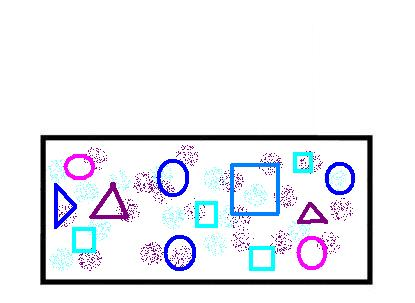
\includegraphics[height=4cm]{kuch.jpg}
\caption[Beispiel f"ur einen Kuchen]{Ein rechteckiger Kuchen mit unterschiedlichen Merkmalen vgl.\cite{25}. Die einzelnen Fragmente sind unterschiedlich wertvoll f"ur die Spieler.}
\end{figure} Die Division wird durch eine Reihe von parallen Schnitten durchgef"uhrt.\footnote{Es gibt ebenfalls Aufteilungen mit parallelen und rechtwinkligen Schnitten (z.B. Protokoll von Webb).} Der Kuchen $X$ wird dabei durch das Intervall $I=[0,1]\subseteq \mathbb{R}$ repr"asentiert. Jedes Teilintervall $I'\subseteq I$, oder eine Vereinigung von solchen, wird als \underline{St"uck} bezeichnet. Diese St"ucke sind immer disjunkt. Das St"uck des Kuchens, welches der Spieler $p_i$ bekommt, wird \underline{Portion} genannt und als $X_i$ bezeichnet. Jedes St"uck hat eine objektive L"ange, welche der Summe der Differenzen seiner Grenzen entspricht und eine subjektive Bewertung, die folgend entsteht:\\
\newline
\textbf{Die Bewertung} \\
\newline
Jeder Spieler $p_i \in P_N$ besitzt eine Bewertungsfunktion (Bewertung) $v_i:\{X'|X'\subseteq X\}\mapsto [0,1]$ des Kuchens $X$. Sie erf"ullt folgende Eigenschaften\footnote{vgl. zus"atzlich \cite{24}}:
\begin{enumerate}
\item Nicht-Negativit"at\footnote{manchmal auch Positivit"at: $v_i(C)> 0$ f"ur alle $C\subseteq [0,1], C \neq \emptyset.$}: $v_i(C)\geq 0$ f"ur alle $C\subseteq [0,1].$
\item Normalisierung: $v_i(\emptyset)=0$ und $v_i([0,1])=1.$
\item Monotonit"at: Wenn $C' \subseteq C$, dann $v_i(C') \leq v_i(C).$
\item Additivit"at: $v_i(C \cup C')=v_i(C)+v_i(C')$ f"ur disjunkte $C,C'\subseteq [0,1].$
\item Teilbarkeit: F"ur alle $C\subseteq [0,1]$ und alle $\alpha \in \mathbb{R}$, $0\leq \alpha \leq 1$, existiert ein $B\subseteq C$, so dass  $v_i(B)=\alpha \cdot v_i(C).$
\item  $v_i$ ist kontinuierlich: Falls $0<x<y\leq 1$ mit $v_i([0,x])=\alpha$ und $v_i([0,y])=\beta$, dann gilt f"ur jedes $\gamma \in [\alpha,\beta]$ existiert ein $z \in [x,y]$ so dass $v_i([0,z])=\gamma.$
\item Inhaltslosigkeit von Punkten:  $v_i([x,x])=0$ f"ur alle $x\in [0,1].$
\end{enumerate}
Bei den Beispielen wird die folgende Darstellung f"ur den Kuchen und deren Bewertung genutzt:\\
\newline
Die \textbf{Boxendarstellung}:
\begin{figure}[h!]
\center
 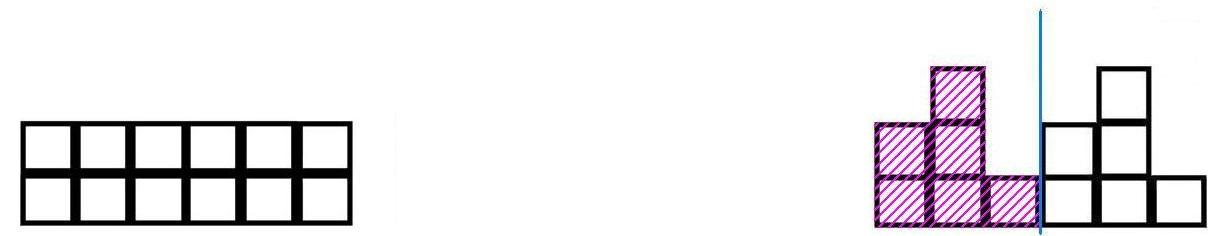
\includegraphics[height=3cm]{cc1svv.jpg}
\caption[Beispiel f"ur die Boxendarstellung eines Kuchens]{Eigenschaften: Ein solches Diagramm muss separat f"ur jeden Spieler erstellt werden. Die Anzahl der K"astchen ist bei allen Spielern gleich und diese repr"asentieren immer den gleichen Wert des Kuchens. Ab hier wird der Wert des Kuchens pro K"astchen genau $1/12$ und er wird linear auf der Fl"ache des K"astchens verteilt, z.B: 1/2 K"astchen = 1/24 der Kuchens. Die L"ange des Kuchens ist bei allen Spielern einheitlich sechs K"astchen. Diese Einschr"ankungen der Eigenschaften werden gemacht um die Beispiele verst"andlicher und einfacher zu machen. Der objektive Wert eines Kuchens sieht wie die linke Abbildung aus. Es werden die zw"olf K"astchen nach der jeweiligen Bewertung des Spieler verteilt, wie z.B. in der rechten Abbildung. Die straffierte Fl"ache ist das St"uck, welches der jeweilige Spieler erh"alt und dessen Summe ist der Wert seines St"uckes. Die parallelen Schnitte werden wie abgebildet eingezeichnet.}
\end{figure}
\newline
\textbf{Die unterschiedlichen Arten von Gerechtigkeit}\\
\newline
Wie oben bereits definiert wurde, besitzt jeder Spieler eine Bewertungsfunktion. Diese Funktion ist geheim und subjektiv (ein Spieler kennt nur seine Bewertungen, und nur seine Bewertungen haben Einfluss auf sein Wohlbefinden). Nach einer Aufteilung wird die G"ute dieser gemessen. Daf"ur werden Ma"sst"abe ben"otigt. Der Wichtigste ist die Gerechtigkeit. Aber was bedeutet "uberhaupt gerecht? Dies ist eine philosophische oder psychologische Frage und kann nicht so einfach und f"ur das gegebene Ziel zufriedenstellend beantwortet werden. Also werden Kriterien ben"otigt um die Aufteilungen untereinander vergleichen und bewerten zu k"onnen. Alle Kriterien sind als subjektive Einsch"atzungen von den Spielern und nicht alss objektive Ma"sst"abe zu verstehen. 
\begin{defi}{\textbf{(Proportionalit"at oder einfache Gerechtigkeit)}}
\newline Eine Aufteilung ist \underline{proportional (einfach gerecht)}, falls  $v_i(X_i) \geq 1/n$ f"ur jeden Spieler $p_i \in P_N$ gilt. 
\end{defi} 
\begin{defi}{\textbf{(Neidfreiheit)}}
\newline Eine Aufteilung ist \underline{neidfrei}, falls $v_i(X_i) \geq v_i(X_j)$ f"ur jedes Paar von Spielern $p_i, p_j \in P_N$. 
\end{defi}
\begin{defi}{\textbf{(Starke Neidfreiheit)}}
\newline  Eine Aufteilung ist \underline{stark-neidfrei} falls $v_i(X_i) > v_i(X_j)$ f"ur jedes Paar von Spielern $p_i, p_j \in P_N, i \neq j$.  
\end{defi} 
\begin{defi}{\textbf{(Super Neidfreiheit)}}
\newline Eine Aufteilung ist \underline{super-neidfrei}, falls $v_i(X_j) \leq 1/n$  f"ur jedes Paar von Spielern $p_i, p_j \in P_N, i \neq j$. 
\end{defi} 
\begin{defi}{\textbf{(Starke Super Neidfreiheit)}}
\newline Eine Aufteilung ist \underline{stark-super-neidfrei}, falls $v_i(X_j) < 1/n$  f"ur jedes Paar von Spielern $p_i, p_j \in P_N, i \neq j$. 
\end{defi} 
Das Problem ist, dass f"ur die st"arkeren Einschr"ankungen nicht immer Aufteilungen existieren, z.B. wenn alle Spieler die gleiche Bewertungsfunktion auf den Kuchen besitzen. 
\begin{defi}{\textbf{(Exaktheit)\footnote{In der Literatur wird an Stelle von Exaktheit oft der Begriff der Gerechtigkeit verwendet, was in gewissem Sinne den gesamten Konzept der Begriffe widerspricht, da alle diese Kriterien einzeln als unterschiedliche Ma"sst"abe von gerecht befunden werden.}}}
\newline Eine Aufteilung ist \underline{exakt}, falls $v_i(X_i) = v_j(X_j)$ f"ur jedes Paar von Spielern $p_i, p_j \in P_N$.
\end{defi}
In wirtschaftlichen Texten werden Aufteilungen, die gleichzeitig exakt und neidfrei, sind oft als besonders gerecht empfunden. Dennoch hat die Exaktheit sogar in Kombination mit der Proportionalit"at keinen direkten Zusammenhang mit der Neidfreiheit, wie man sich am folgenden Beispiel leicht veranschaulichen kann.\\
\begin{bsp}Die Spieler Aleph, Beth und Gimel teilen einen Kuchen. Am Ende bekommt jeder Spieler genau $1/3$ des Kuchens (nach seinem Ma"s). Diese Aufteilung ist exakt und proportional. Doch Aleph ist der Meinung, dasgBeths St"uck genau die H"alfte des Kuchens ist und beneidet Beth. Damit ist die Aufteilung nicht neidfrei.\end{bsp}
\textbf{Zusammenh"ange der Gerechtigkeitskriterien:}
\begin{lem}
F"ur alle Aufteilungen gilt:
\begin{enumerate}
\item Falls eine Aufteilung neidfrei ist, so ist sie auch proportional.
\item F"ur zwei Spieler ist eine Aufteilung proportional genau dann, wenn sie neidfrei ist.
\end{enumerate}
\end{lem}
\begin{proof}\wf jhbfd \tf
\begin{enumerate}
\item Beweis durch Widerspruch:\\ Sei $A$ eine Aufteilung die neidfrei, aber nicht proportional ist. Da die Aufteilung $A$ neidfrei ist, gilt $v_i(X_i) \geq v_i(X_j)$ f"ur jedes Paar von Spielern $p_i, p_j \in P_N$ und somit hat jeder Spieler mind. soviel wie jeder andere. Daraus folgt, dass jeder Spieler mindestens genauso viel wie $(n-1)$ andere hat und somit mindestens $1/n$. Damit ist die Aufteilung $A$ proportional. $\lightning$\\Somit sind alle neidfreien Aufteilungen proportional.
\item ''$\Rightarrow$'' F"ur zwei Spieler ist eine Aufteilung proportional, wenn er mind. die H"alfte des Kuchens bekommt, damit kann der andere Spieler h"ochstens die H"alfte bekommen und wird nicht beneidet.\\ ''$\Leftarrow$'' Die R"uckrichtung folgt aus Zusammenhang 1.\\
\end{enumerate}
\end{proof}
\begin{defi}{\textbf{(Effizienz)}}
\newline Eine Aufteilung ist \underline{effizient (Pareto optimal)}, falls keine andere Aufteilung existiert, die einem Spieler ein von ihm besser bewertetes St"uck einbringt, ohne die Situation eines anderen Spielers zu verschlechtern. 
\end{defi}
\begin{defi}{\textbf{(Ehrlichkeit)\footnote{In den letzten Jahren wurde dieser Aspekt konzentrierter untersucht vgl. \cite{23}. Es kann als ein einzelnes Kriterium formuliert werden.}}}
\newline Eine Aufteilung (Prozedur) ist \underline{ehrlich}, falls es keine Bewertungen gibt, bei der Spieler am Ende durch Unaufrichtigkeit ein wertvolleres St"uck bekommen h"atten. \footnote{''We say that a cake cutting procedure is truthful iff there are no valuations where a player will do better by lying.'' aus \cite{41}.}
\end{defi}
Es besteht nur Interesse an Aufteilungen, wo die Ehrlichkeit die beste Strategie f"ur alle Spieler ist und somit allein durch den Algorithmus erzwungen wird. Oft wird dies erreicht, indem der Spieler durch Unaufrichtigkeit Gefahr l"auft die Garantie auf seinen gerechten Anteil zu verlieren.\\
\subsection{Grundbegriffe der Komplexit"atsanalyse von Protokollen}
\textbf{Komplexit"atsklassen\footnote{aus \cite{19}}}\\
\newline
Um Algorithmen anhand ihrer Laufzeiten besser zuordnen und vergleichen zu k"onnen wurden die zwei nachfolgenden Funktionenklassen eingef"uhrt.
$$\mathcal{O}(g)= \{f :\mathbb{N} \mapsto \mathbb{N} | (\exists c >0)(\exists n_0 \in \mathbb{N}) (\forall n \geq n_0) [f(n) \leq c \cdot g(n)]\}$$
 Die Funktion $f \in \mathcal{O}(g)$ w"achst asymptotisch nicht schneller als $g$. Es d"urfen Konstanten und endlich viele Ausnahmen vernachl"assigt werden. Die Funktion $g$ wird als \underline{obere Schranke} bezeichnet. In dieser Funktionsklasse liegt immer der \underline{ung"unstigste Fall}. Dies ist eine g"ultige Eingabe, f"ur dessen L"osung der Algorithmus die l"angste Zeit ben"otigt. \\
$$\Omega(g)= \{f :\mathbb{N} \mapsto \mathbb{N} | (\exists c >0)(\exists n_0 \in \mathbb{N}) (\forall n \geq n_0) [f(n) \geq c \cdot g(n)]\}$$
 Die Funktion $g$ w"achst asymptotisch nicht schneller als jedes $f \in \Omega(g)$. Die Funktion $g$ wird als \underline{untere Schranke} bezeichnet. In dieser Funktionsklasse liegt immer der \underline{beste Fall}. "Ublicherweise ist diese Zeitangabe kleiner als das tats"achliche Resultat, aber man kann beweisen, dass ohne diesen Zeitaufwand das Problem nicht l"osbar ist.\\
\newline
\textbf{Klassen von Protokollen}\\
\newline
Intuitive Beschreibung: \underline{Algorithmus}
\newline In der Mathematik, Informatik und verwandten Gebieten, ist ein Algorithmus eine effektive Methode zur Probleml"osung, ausgedr"uckt durch eine endliche Folge von Anweisungen.
\begin{defi}{\textbf{(Protokoll (Cake-Cutting-Protokoll)\footnote{Vgl. mit Definition aus \cite{3}, \cite{35} und \cite{24} oder \cite{34}\abk{CC}{\markup{C}ake-\markup{C}utting}.}
)}}
\newline Ein \underline{Protokoll (Cake-Cutting-Protokoll)} ist ein Algorithmus mit mehreren Spielern und folgenden Eigenschaften:
\begin{itemize}
\item{Es besteht aus Regeln und Strategien.\\ \underline{Regeln} sind Anweisungen, die gefordert werden ohne die Bewertungen der Spieler zu kennen.\\ \underline{Strategien} sind Empfehlungen, welchen der Spieler folgen muss um garantiert seinen gerechten Anteil zu bekommen.
}
\item{Sofern ein Spieler sich nicht an die Strategie des Protokolls h"alt, verliert er seinen Anspruch nach einer endlichen Anzahl von Schritten ein St"uck des Kuchens zu bekommen, welches dem geforderten Gerechtigkeitskriterium entspricht. Sein Vorgehen hat aber keine Auswirkungen auf die Anteile der anderen Spieler.}
\item Jeder Spieler muss zu jeder Zeit in der Lage sein, v"ollig unabh"angig von den anderen Spielern den Kuchen zu teilen (einen Schnitt zu machen).
\item Das Protokoll besitzt keine Informationen "uber die Bewertungen der Spieler, ausser denen die angefragt wurden in dem jeweiligen oder in den vorherigen Schritten.\footnote{Diese Eigenschaft ist wichtig f"ur die Komplexit"atsanalyse.}
\end{itemize}
\end{defi}
\begin{defi}
Ein Cake-Cutting-Protokoll wird proportional, neidfrei, stark neidfrei etc. genannt, falls unabh"angig von den Bewertungsfunktionen der Spieler, jede Aufteilung entsprechend proportional, neidfrei etc., unter der Vorraussetzung, dass alle Spieler die vom Protokoll vorgegebenen Regeln und Strategien befolgen, ist.
\end{defi}
Eines der Ziele von Cake-Cutting ist solche Protokolle anzugeben.\begin{defi}{\textbf{(endlich (diskret)/kontinuierlich)}}
\newline Ein \underline{endliches (diskretes)} Protokoll liefert eine L"osung nach einer endlichen Anzahl von Entscheidungen (Bewertungen, Markierungen,$\ldots$), dagegen muss ein Spieler bei einem \underline{kontinuierlichen} Protokoll unendlich viele Entscheidungen treffen.
\end{defi}
\begin{defi}{\textbf{(endlich beschr"ankt/endlich unbeschr"ankt))}}
\newline Ein \underline{endlich beschr"anktes} Protokoll hat eine obere Grenze von Schritten, welche im ung"unstigsten Fall betrachtet wird. Die gesamte Anzahl von Entscheidungen h"angt, wenn "uberhaupt, dann nur von der Anzahl der beteiligten Personen ab. Ein \underline{endlich unbeschr"anktes} Protokoll hat hingegen eine nicht im Voraus absch"atzbare Anzahl.
\end{defi}
Die begehrtesten Protokolle sind endlich beschr"ankt, da sie am einfachsten in der Realit"at umsetzbar sind. Aber es gibt eine Art von kontinuierlichen Protokollen, an denen ebenfalls Interesse besteht.
\begin{defi}{\textbf{(Moving-Knife-Protokoll)}}
\newline Ein Schiedsrichter, welcher unparteisch gegen"uber den Spielern ist und unbeteiligt an der Verteilung der St"ucke, \underline{schwenkt ein Messer kontinuierlich} von links nach rechts und macht parallele Schnitte sofern ein Spieler ''Halt!'' ruft. Bei manchen MKP\abk{MKP}{\markup{M}oving-\markup{K}nife-\markup{P}rotokoll} wird der Schiedsrichter ausgelassen und nur ein Messer oder Schwert geschwungen.
\end{defi}
Bemerkung: In der Literatur (z.B.: \cite{36}) werden manchmal kontinuierliche Protokolle nicht als Protokolle bezeichnet sondern zu neuen Klassen zusammengefasst, die von der Anzahl der Messer abh"angen.\\
\newline
 Eine weitere wichtige Eigenschaft von Cake-Cutting ist, dass nur komplette Aufteilungen des Kuchens,also wo jedes St"uck einem Spieler zugeordnet wird, betrachtet werden.
\newpage
\section{Neidfreie Cake-Cutting-Protokolle}
\textbf{Bekannte Ergebnisse:}\\
Die neidfreie Aufteilung wurde f"ur bis zu vier Spieler im kontinuierlichen und bis zu drei Spieler im endlich beschr"ankten Fall gel"ost. Es gibt ein endliches Protokoll f"ur beliebig viele Spieler. Dieser unterscheidet sich stark von den bisherigen und ist nicht endlich beschr"ankt, vgl. \cite{5}. Es gibt mehrere fast neidfreie L"osungen, siehe dazu \cite{11} und \cite{12}.
\\Es folgen wichtige neidfreie Cake-Cutting-Protokolle\abk{CCP}{\markup{C}ake-\markup{C}utting-\markup{P}rotokoll}. Diese sind mit Ausnahme von AMKP f"ur $n$ Spieler und dem exakten Protokoll aus den B"uchern \cite{26} und \cite{27} und der Vorlesung \cite{28} entnommen. Bei den Protokollen wird erl"autert, wie die Neidfreiheit erreicht wird und begr"undet, woran eine Verallgemeinerung scheitert. Au"serdem wird nach M"oglichkeit an einem Beispiel die Funktionsweise gezeigt. Es werden nur Protokolle f"ur einen rechteckigen Kuchen mit parallelen Schnitten betrachtet.
\subsection{Zwei Spieler}
Es folgt das intuitivste und bekannteste endlich beschr"ankte CCP, das eine neidfreie Aufteilung liefert. Es werden ein Schnitt und eine Bewertung gemacht.\\
\newline
\begin{tabular}{|ll|}
\hline
&\textbf{Cut \& Choose-Protokoll}\wf ergrgrgevdffergdtdfvdjgujzgvjuvnkwgttvgvtrbr\tf\\
\hline
\textbf{$\cdot$ Schritt 1}&Spieler $p_1$ schneidet den Kuchen in zwei gleichwertige Teile\\&(nach seinem Ma"s).\\
\textbf{$\cdot$ Schritt 2}&Spieler $p_2$ sucht sich ein St"uck aus, das andere St"uck bekommt Spieler $p_1$.\\
\hline
\end{tabular}
\newline
\newline
\newline
Die Neidfreiheit wird elementar erreicht, da der erste Spieler zufrieden mit jedem der zwei St"ucke ist, und der andere Spieler das Privileg hat zu w"ahlen. Eine Verallgemeinerung ist ausgeschlossen, da das Verfahren nur dadurch funktioniert, dass der jeweils andere Spieler den Rest des Kuchens von dem jeweiligen Spieler bekommt.\\Bemerkung: Der erste Spieler kann nie mehr als die H"alfte des Kuchens bekommen.
\begin{bsp}\wf rfsdf
\begin{figure}[h!]
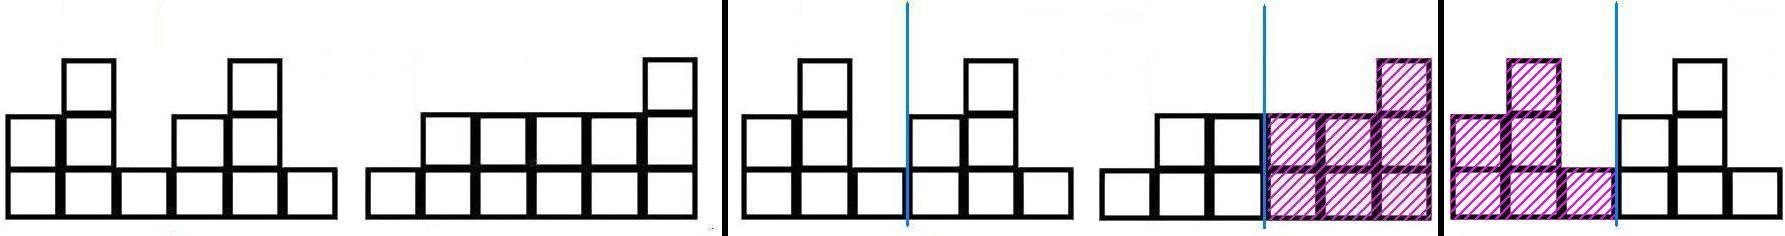
\includegraphics[height=2cm]{cc3.jpg}
\caption[Beispiel zum Cut \& Choose-Protokoll]{Boxendarstellungen des Kuchens f"ur die Spieler $p_1$ (links) und $p_2$ (rechts); Spieler $p_1$ halbiert den Kuchen(n.s.M.) (links) und Spieler $p_2$ w"ahlt das wertvollere St"uck (rechts); Spieler $p_1$ bekommt das "ubriggebliebene St"uck}
\end{figure}
\end{bsp}
Es folgt ein kontinuierlich beschr"anktes, exaktes und neidfreies CCP. Es werden h"ochstens zwei Schnitte gemacht.\\
\newline
\begin{tabular}{|ll|}
\hline
&\textbf{Austin Moving-Knife-Protokoll}\wf ergrgrgergegetdfvafvvvadfffrgergvtrf\tf\\
\hline
\textbf{$\cdot$ Schritt 1}& Ein Messer wird kontinuierlich von links nach rechts "uber den Kuchen\\&geschwenkt, bis ein Spieler (sei dies Spieler $p_1$) :''Halt!'' ruft, weil das Messer\\&den Kuchen dort halbiert (nach seinem Ma"s).\\
\textbf{$\cdot$ Schritt 2}& Dieser Spieler platziert ein zweites Messer "uber dem linken Rand des\\&Kuchens und schwenkt beide Messer parallel und kontinuierlich von links\\&nach rechts so "uber den Kuchen, dass zwischen ihnen (nach seinem Ma"s)\\&stets der Wert des Kuchens $1/2$ ist.\\
\textbf{$\cdot$ Schritt 3}& Der andere Spieler ruft:''Halt!'', sobald der Wert dieses St"uckes $1/2$ erreicht.\\
\hline
\end{tabular}
\newline
\newline
\newline
 Dieses Protokoll ist neidfrei, da jeder der Spieler genau die H"alfte des Kuchens bekommt (nach seinem Ma"s).\\Die Idee: Wenn der erste Spieler ''Halt!'' ruft, ist das St"uck vom linken Rand bis zum Messer f"ur den zweiten Spieler weniger Wert als die H"alfte des Kuchens (sonst w"urde er auch: ''Halt!'' rufen und damit w"are das gew"unschte Ergebnis bereits erzielt). Daraus folgt, dass das St"uck von dem Messer bis zu dem rechten Rand f"ur den zweiten Spieler mehr Wert hat als die H"alfte des Kuchens. Da der erste Spieler nun aber mit zwei Messern aus dem linken St"uck in das rechte St"uck "ubergeht, ist gesichert, dass es einen Zeitpunkt gibt, wo das St"uck zwischen den beiden Messern genau die H"alfte des Kuchens f"ur den zweiten Spieler ist.\\
Bis jetzt konnte kein Protokoll aufgestellt werden, welches f"ur $n>2$ Spieler eine Aufteilung in zwei gleichwertvolle St"ucke liefert.
\begin{bsp}\wf rfsdf
\begin{figure}[h!]
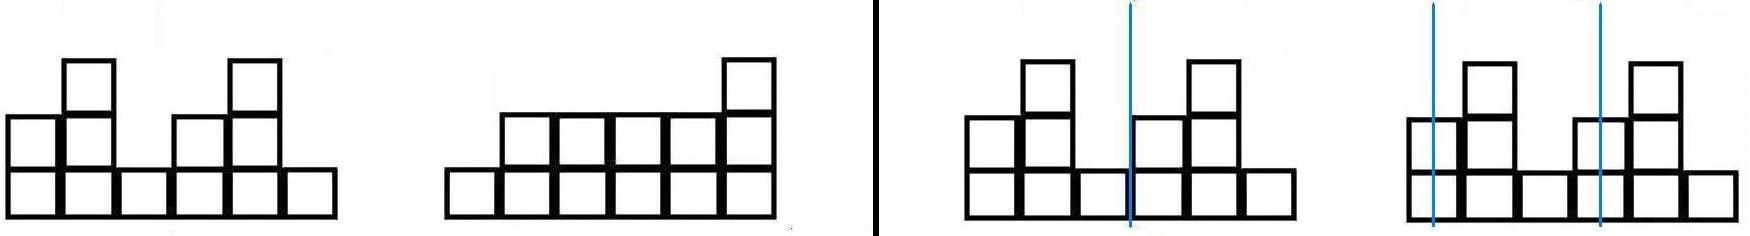
\includegraphics[height=2cm]{cc4.jpg}
\caption[Beispiel zum Austin Moving-Knife-Protokoll 1/2]{Boxendarstellungen des Kuchens f"ur die Spieler $p_1$ (links) und $p_2$ (rechts); Spieler $p_1$ ruft:''Halt!'' wenn die H"alfte erreicht wird (links), und f"ugt ein zweites Messer hinzu und schwenkt diese "uber den Kuchen (rechts)}
\end{figure}
\begin{figure}[h!]
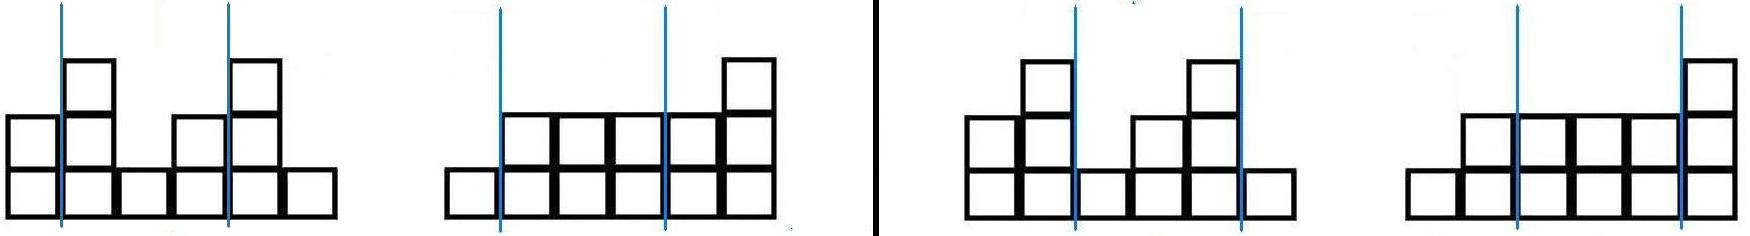
\includegraphics[height=2cm]{cc5.jpg}
\caption[Beispiel zum Austin Moving-Knife-Protokoll 2/2]{Spieler $p_2$ ruft: ''Halt!''. Beide St"ucke haben zwischen den Messern den Wert $1/2$; Die Situation in Schritt 3 ist nicht eindeutig! Der erste Zustand in dem der Wert des Kuchens f"ur beide Spieler zwischen den Messern $1/2$ ist, gilt als Ergebnis der Aufteilung.}
\end{figure}
\end{bsp}
Diese Prozedur funktioniert auch f"ur jedes beliebige $1/n$ mit $n \in \mathbb{N}$ nach der Aussage von Austin aus \cite{20}, muss aber im ung"unstigsten Fall $(n-1)$- mal durchgef"uhrt werden. Denn es entsteht nach jeder Durchf"uhrung ein Restst"uck, welches zur n"achsten Durchf"uhrung "ubertragen werden muss. Es folgt die Bemerkung von Austin als ausgeschriebenes Protokoll:\\
\newline
\begin{tabular}{|ll|}
\hline
&\textbf{Austin Moving-Knife-Protokoll f"ur $n$ gleichwertige St"ucke}\wf gfdffgsa\tf\\
\hline
\textbf{$\cdot$ Schritt 1}& Der Spieler $p_1$ schneidet den Kuchen in $n$ gleichwertige St"ucke (n.s.M.)\abk{n.s.M.}{\markup{n}ach \markup{s}einem \markup{M}ass}.\\
\textbf{$\cdot$ Schritt 2}& Der Spieler $p_2$ w"ahlt zwei St"ucke $\{X_1,X_2\}$ davon aus mit der Eigenschaft:\\&$v_2(X_1) \leq 1/n,v_2(X_2) \geq 1/n$. Alle St"ucke mit $v_2(X_i)=1/n$ f"ur $3\leq i \leq n$\\&werden als fertig markiert und stehen nicht mehr zur Wahl.\\
\textbf{$\cdot$ Schritt 3}& Diese zwei St"ucke $\{X_1,X_2\}$ werden zu einem verschmolzen und darauf\\&wird das Austin Moving-Knife-Protokoll angewendet. Das resultierende\\&St"uck wird ebenfalls als fertig markiert. Der Rest wird zu einem\\&St"uck verschmolzenund zu den "ubrigen unfertigen St"ucken zugeordnet,\\&sofern einer der beiden Spieler es nicht als $1/n$ bewertet.\\
\textbf{$\cdot$ Schritt 4}& Schritt 2 und Schritt 3 werden wiederholt, bis alle St"ucke markiert sind.\\
\hline
\end{tabular}
\begin{bsp}\wf rfsdf 
\begin{figure}[h!]
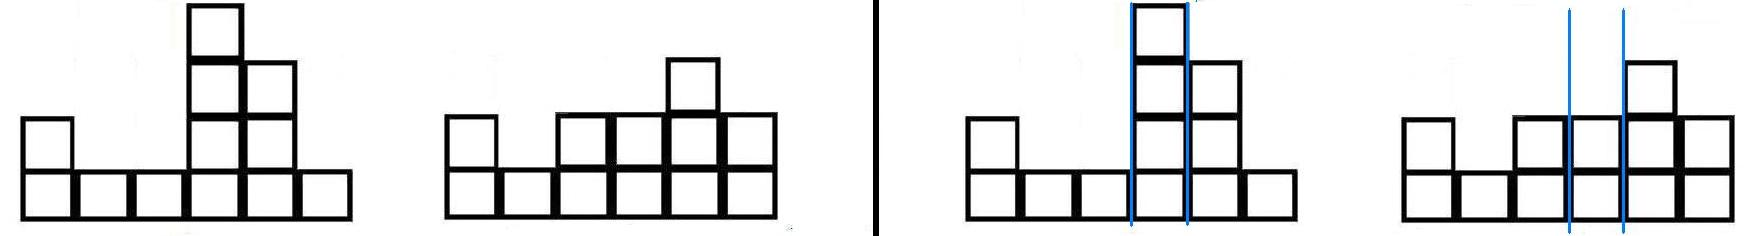
\includegraphics[height=2cm]{cc7.jpg}
\caption[Beispiel zum Austin Moving-Knife-Protokoll f"ur 3 gleichwertige St"ucke 1/2]{Boxendarstellungen des Kuchens f"ur die Spieler $p_1$ (links) und $p_2$ (rechts); Spieler $p_1$ schneidet den Kuchen in 3 gleichwertige St"ucke (n.s.M)(links)}
\end{figure}
\begin{figure}[h!]
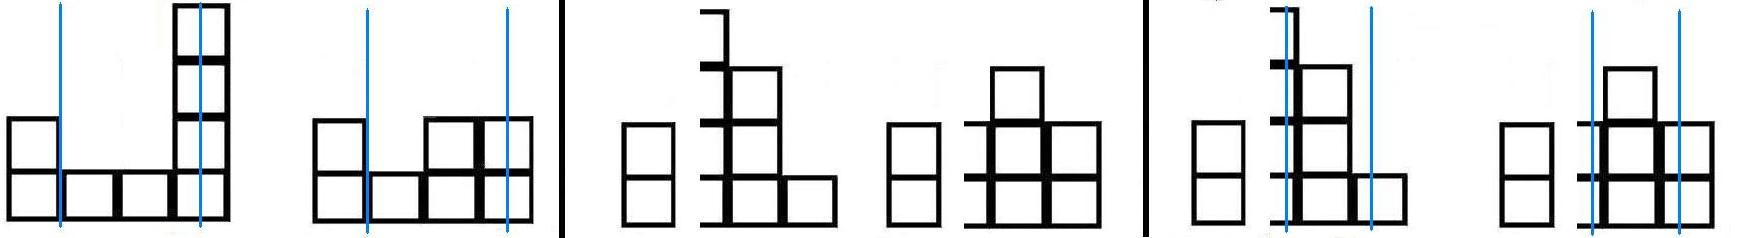
\includegraphics[height=2cm]{cc9.jpg}
\caption[Beispiel zum Austin Moving-Knife-Protokoll \abk{AMKP}{\markup{A}ustin \markup{M}oving-\markup{K}nife-\markup{P}rotokoll} f"ur 3 gleichwertige St"ucke 2/2]{Spieler $p_2$ sucht sich 2 St"ucke aus mit der geforderten Eigenschaft aus Schritt 2. Beide Spieler f"uhren AMKP aus. Dadurch entsteht ein St"uck, welches beide Spieler gleich bewerten (zwischen den Schnitten); Das andere St"uck ist nicht gleich bewertet worden, also wird es zusammengesetzt und als unfertiges St"uck markiert. Es wird das n"achste St"uck dazu genommen (mitte); AMKP wird ausgef"uhrt (rechts)}
\end{figure}
\end{bsp}
\subsection{Drei Spieler}
Es folgt ein endlich beschr"anktes, neidfreies CCP. Es werden h"ochstens f"unf Schnitte gebraucht. Dies ist das einzige bekannte endlich beschr"ankte neidfreie Protokoll f"ur $n \geq 3$.\\
\newline
\begin{tabular}{|ll|}
\hline
&\textbf{Selfridge-Conway-Protokoll}\wf jsngkdbfkhbdfbdfffkrgergergbdhljbfngk\tf\\
\hline
\textbf{$\cdot$ Schritt 1}&Der erste Spieler $p_1$ schneidet den Kuchen $X$ in drei gleiche St"ucke\\&(nach seinem Ma"s). Der zweite Spieler $p_2$ sortiert $\{X_1,X_2,X_3\}$ mit:\\
& $v_1(X_1)=v_1(X_2)=v_1(X_3)=1/3$ und $v_2(X_1) \geq v_2(X_2) \geq v_2(X_3)$.\\
\textbf{$\cdot$ Schritt 2}& Ist $v_2(X_1)>v_2(X_2)$, so schneidet $p_2$ von $X_1$ etwas ab, so dass er\\&$X_1'=X_1-R$ erh"alt mit   $v_2(X_1')=v_2(X_2)$. Ist $v_2(X_1)=v_2(X_2)$,\\&so sei $X_1'=X_1$.\\
\textbf{$\cdot$ Schritt 3}&Aus $\{X_1',X_2,X_3\}$ w"ahlen $p_3,p_2,p_1$ in dieser Reihenfolge je ein St"uck.\\&Wenn $p_3$ $X_1'$ nicht nimmt, muss $p_2$ es tun.\\
\textbf{$\cdot$ Schritt 4}& Entweder $p_2$ oder $p_3$ hat $X_1'$. Nenne diesen Spieler\\(nur falls $R \neq \emptyset$)&$P$, den anderen $Q$. $Q$ schneidet den Rest $R$ in drei gleiche St"ucke\\&(nach seinem Ma"s): $v_Q(R_1)=v_Q(R_2)=v_Q(R_3)=1/3 \cdot R$\\& $P,p_1,Q$ w"ahlen in dieser Reihenfolge je ein St"uck.\\
\hline
\end{tabular}
\newline
\newline
\newline
 Um zu zeigen, dass die erste Aufteilung von $X-R$ neidfrei ist, werden alle Spieler und ihre Portionen einzeln betrachtet. Der dritte Spieler hat die freie Wahl sich das wertvollste St"uck zu nehmen (n.s.M.) und kann somit keinen beneiden, f"ur den zweiten Spieler existieren zwei St"ucke und da er als zweiter w"ahlen darf, ist eines davon immer vorhanden. Der erste Spieler bekommt ein unbeschnittenes St"uck und ist somit der Meinung, dass die anderen entweder gleichgrosse oder kleinere St"ucke als er haben. Danach wird, falls n"otig, der Rest $R$ verteilt, hier ist der erste Spieler der Meinung, dass der gesamte Rest eigentlich dem Spieler $P$ geh"ort und hat kein Problem diesen als ersten w"ahlen zu lassen. Damit beneidet $P$ niemanden, denn er durfte sich (nach seinem Ma"s) das gr"osste St"uck aussuchen. Der Spieler $p_1$ w"ahlt nun sein St"uck und kann den Spieler $Q$ nicht beneiden. Weiterhin ist Spieler $Q$ der Meinung, dass alle Restst"ucke waren gleich gross, und damit ist $R$ neidfrei aufgeteilt. Da auch $X-R$ neidfrei aufgeteilt wurde folgt mit der Additivit"at von Bewertungen, dass die gesamte Aufteilung neidfrei ist.\\
Die Verallgemeinerung scheitert vor allem an der zweiten Aufteilung. Der erste Teil l"asst sich als das unendliche Protokoll in Kapitel 4.4 formulieren. Aber bereits hier entsteht das Problem mit den Resten. Bei mehr als drei Spieler braucht der zweite Spieler mindestens drei gleichwertige St"ucke und m"usste damit eventuell von zwei St"ucke etwas abschneiden. Damit ergibt sich mehr als ein Rest und eine gesonderte Behandlung f"ur jeden von diesen Resten wird ben"otigt. Bei der Restaufteilung mit mehr als drei Spieler entsteht auch das Problem, dass es zwar immer einen Spieler gibt, welcher der Meinung ist, dass der Rest einem bestimmten Spieler geh"ort, aber es gibt mehr als einen Spieler der diese Meinung nicht teilen muss. Eine kontinuierliche Verallgemeinerung auf vier Spieler ist das Brams,Taylor \& Zwicker Moving-Knife-Protokoll. 
\begin{bsp}\wf rfsdf
\begin{figure}[h!]
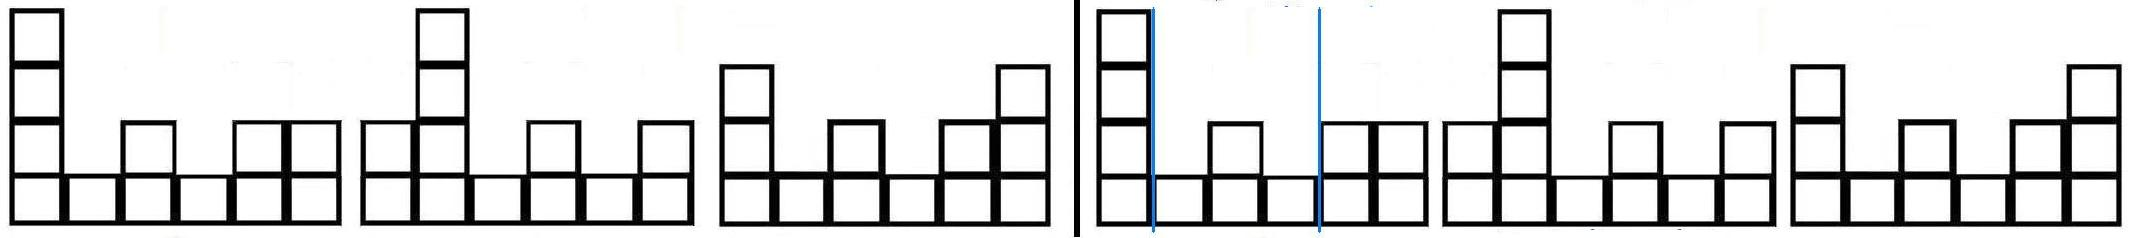
\includegraphics[height=1.73cm]{scc.jpg}
\caption[Beispiel zum Selfridge-Conway-Protokoll 1/3]{Boxendarstellungen des Kuchens f"ur die Spieler $p_1$ (links), $p_2$ (mitte) und $p_3$ (rechts); Der Spieler $p_3$ teilt den Kuchen in 3 gleichwertige St"ucke(n.s.M.)}
\end{figure}
\begin{figure}[h!]
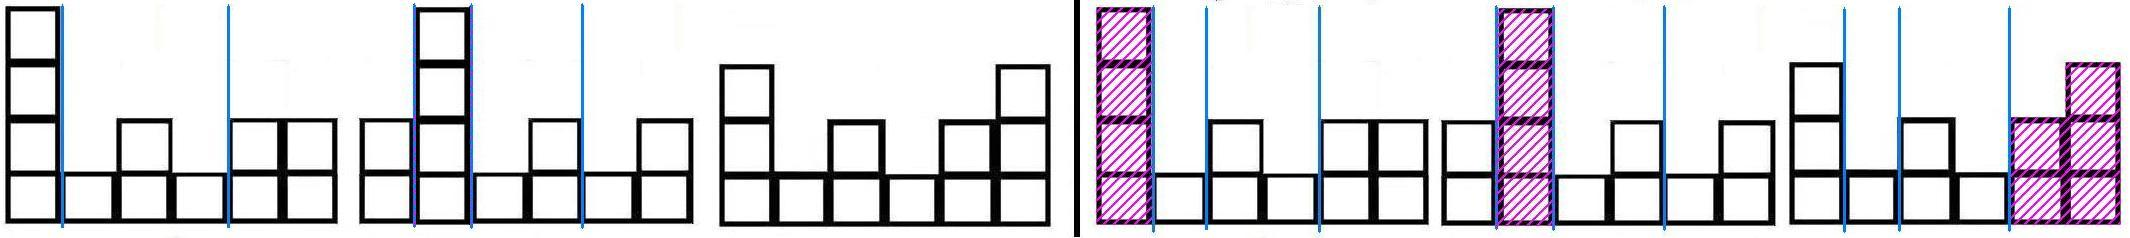
\includegraphics[height=1.75cm]{scc2.jpg}
\caption[Beispiel zum Selfridge-Conway-Protokoll 2/3]{Spieler $p_2$ schneidet etwas von seinem wertvollsten St"uck ab, damit zwei gleichwertvolle St"ucke entstehen; Spieler $p_3$, $p_2$ und $p_1$ w"ahlen in dieser Reihenfolge je ein St"uck}
\end{figure}
\begin{figure}[h!]
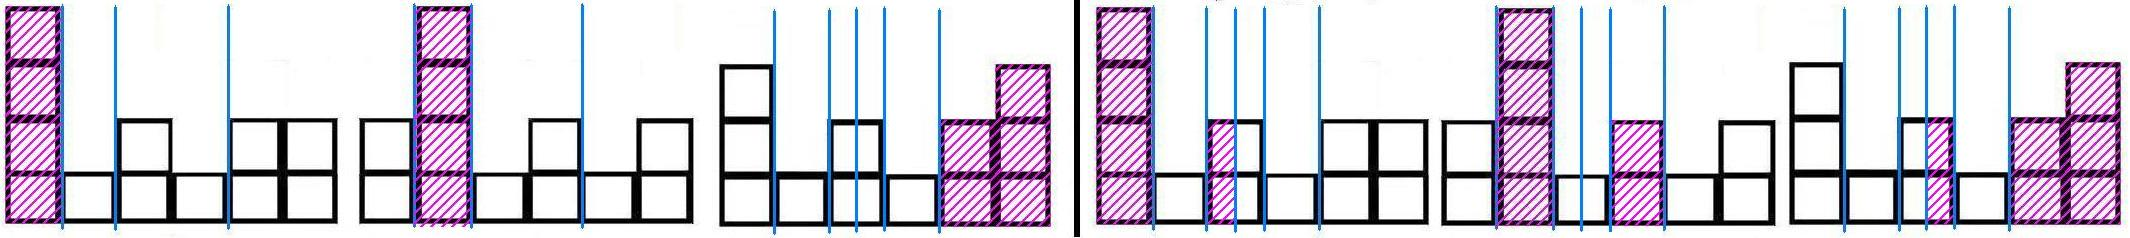
\includegraphics[height=1.75cm]{scc4.jpg}
\caption[Beispiel zum Selfridge-Conway-Protokoll 3/3]{Spieler $p_3$ unterteilt den Rest in 3 gleichwertige St"ucke (n.s.M.); Spieler $p_2$, $p_1$ und $p_3$ w"ahlen in dieser Reihenfolge je ein Restst"uck.}
\end{figure}
\end{bsp}
Es folgt ein kontinuierliches, neidfreies CCP. Es werden zwei Schnitte gemacht.\\
\newline
\begin{tabular}{|ll|}
\hline
&\textbf{Stromquist Moving-Knife-Protokoll}\\
\hline
\textbf{$\cdot$ Schritt 1}& Ein Schwert wird kontinuierlich von links nach rechts "uber den Kuchen\\&geschwenkt und teilt ihn (hypothetisch) in ein linkes St"uck $X_L$ und ein\\&rechtes St"uck $X_R$: $X=X_L\cup X_R$. Jeder der drei Spieler h"alt sein Messer\\&parallel zum Schwert und bewegt es (w"ahrend das Schwert geschwenkt\\&wird) so, dass es das rechte St"uck nach seinem Ma"s stets genau halbiert.\\&Dabei teilt das mittlere der drei Messer $X_R$ in St"ucke:$X_R=X_{RL}\cup X_{RR}$\\
\textbf{$\cdot$ Schritt 2}& Der erste Spieler, der glaubt, $X_L$ sei mindestens so gut wie sowohl $X_{RL}$ als\\&auch $ X_{RR}$, ruft: ''Halt!'' und bekommt $X_L$. Das mittlere der drei Messer\\&schneidet $X_R$ in zwei St"ucke: $X_R=X_{RL}\cup X_{RR}$. Der "ubriggebliebene\\& Spieler, der seine Markierung am n"ahesten an $X_L$ hatte, bekommt $X_{RL}$.\\&Der letzte Spieler bekommt $X_{RR}$.\\     
\hline
\end{tabular}
\newline
\newline
\newline
Um hier die Neidfreiheit nachzuvollziehen, betrachtet man jeden Spieler einzeln. Der Spieler, der ''Halt!'' ruft, ist der Meinung, dass das linke St"uck mehr oder gleich viel wert ist als jedes der beiden St"ucke rechts von dem Schwert, und wird somit auch keinen beneiden. Die "ubrigen zwei Spieler teilen seine Meinung nicht, sonst h"atten sie auch ''Halt!'' gerufen. Nun m"ussen die St"ucke rechts neidfrei verteilt werden. Es gibt drei Markierungen, als Schnitt wird die mittlere genommen. Mindestens einem der "ubrigen Spieler geh"ort eine andere Markierung, damit kriegt er ein St"uck, das sogar noch mehr wert ist als die H"alfte von dem rechten St"uck (n.s.M.) und beneidet den anderen Spieler nicht. F"ur den letzten Spieler gilt entweder exakt das selbe oder er ist der Meinung genauso viel wie der vorherige Spieler bekommen zu haben (sofern seine Markierung die mittlere war). Damit ist die gesamte Aufteilung neidfrei.\\
Die Prozedur l"asst sich leider nicht auf $n \geq 4$ "ubertragen. Entweder wird eine ungerade Anzahl von Spielern ben"otigt, um links ein Schwert zu haben und das rechte St"uck in die entsprechenden Teile zu markieren und eine mittlere Markierung f"ur den Schnitt zu besitzen, oder es werden mehr als ein Schwert verlangt (von links und rechts). Ein solches Konstrukt w"urde den kontinuirlichen Ablauf des Protokolls st"oren. F"ur $n=5$ tritt ein Problem in der Aufteilung der rechten St"ucke auf, da man wieder hier alle Bewertungen von Allen bis auf den Spieler, der das linke  St"uck bekommen hat, beachten muss und man nicht mehr bestimmen kann, welcher Schnitt der mittlere und somit der entscheidende ist.\\
\begin{figure}[h!]
\center
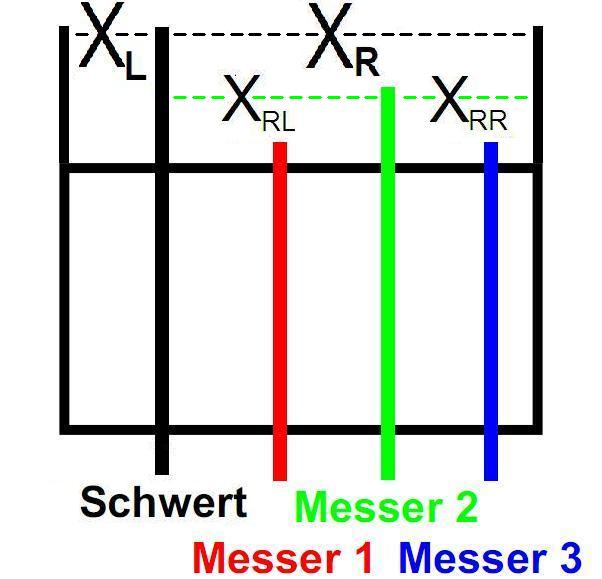
\includegraphics[height=4cm]{str.jpg}
\caption[Vorgehensweise bei Stromquist Moving-Knife-Protokoll]{Die Vorgehensweise bei Stromquist Moving-Knife-Protokoll. Die Markierung von Messer 2 wird zum Schnitt.}
\end{figure}
%\begin{bsp}\wf rfsdf
%\begin{figure}[h!]
%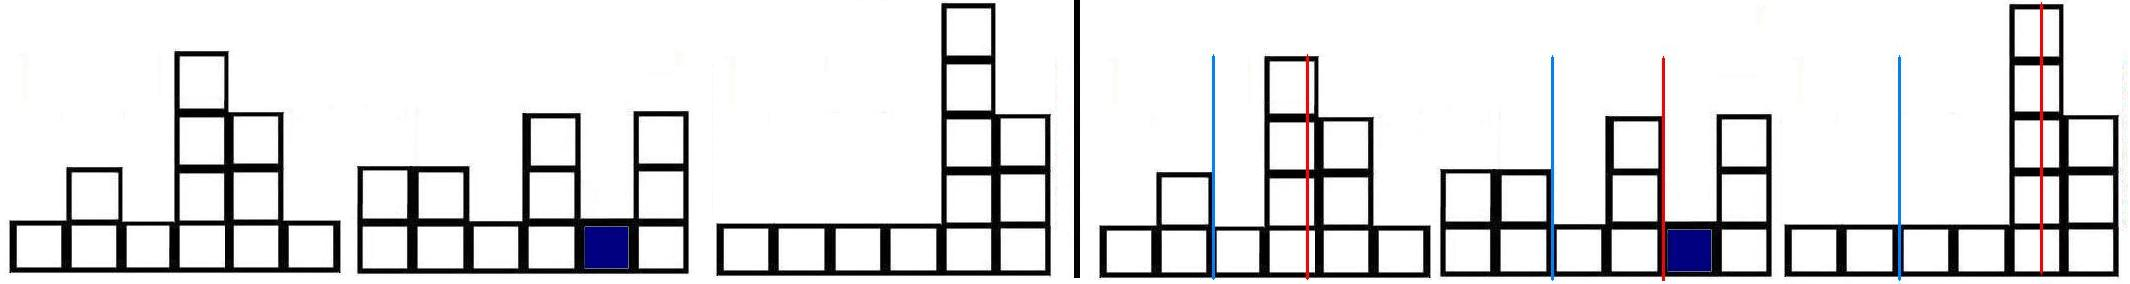
\includegraphics[height=2cm]{st2.jpg}
%\caption[Beispiel zum Stromquist Moving-Knife-Protokoll 1/2] %{Boxendarstellungen des Kuchens f"ur die Spieler $p_1$ (links), $p_2$ %(mitte) und $p_3$ (rechts); Das Schwert wird geschwenkt und die Spieler %halbieren symbolisch das rechte St"uck}
%\end{figure}
%\begin{figure}[h!]
%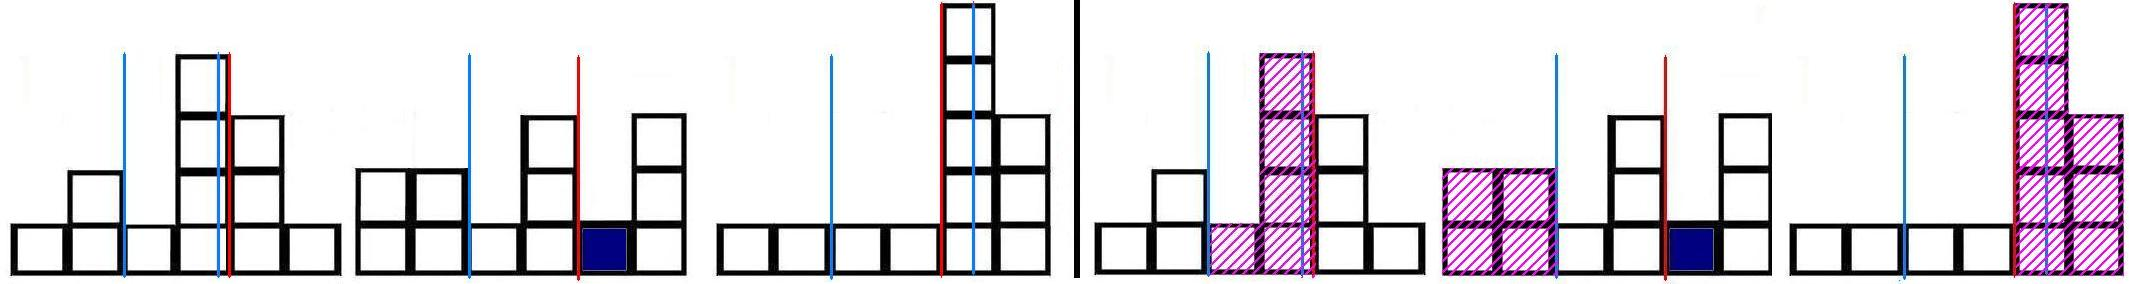
\includegraphics[height=2cm]{st4.jpg}
%\caption[Beispiel beim Stromquist Moving-Knife-Protokoll 2/2]{Spieler %$p_2$ ruft: ''Halt!''; Die St"ucke werden nach dem Protokoll verteilt.}
%\end{figure}
%\end{bsp}
\subsection{Vier Spieler}
Es folgt ein kontinuierliches, neidfreies CCP. Es werden h"ochstens elf Schnitte nach \cite{40} gebraucht. Dies ist das einzige bekannte, beschr"ankte, neidfreie Protokoll f"ur $n \geq 4$.\\ 
\newline
\begin{tabular}{|ll|}
\hline
&\textbf{Brams,Taylor \& Zwicker Moving-Knife-Protokoll}\\
\hline
\textbf{$\cdot$ Schritt 1}&Der erste Spieler $p_1$ und der zweite Spieler $p_2$ erzeugen mit\\&Austin Moving-Knife-Protokoll f"ur beide Spieler vier gleichwertige\\&St"ucke. Der Spieler $p_3$ sortiert diese mit:\\
& $v_1(X_1)=v_1(X_2)=v_1(X_3)=v_1(X_4)=1/4.$\\
& $v_2(X_1)=v_2(X_2)=v_2(X_3)=v_2(X_4)=1/4.$\\
& $v_3(X_1)\geq  v_3(X_2)\geq v_3(X_3)\geq v_3(X_4).$\\
\textbf{$\cdot$ Schritt 2}& Ist $v_3(X_1)>v_3(X_2)$, so schneidet $p_3$ von $X_1$ etwas ab, so dass er\\&$X_1'=X_1-R$ erh"alt mit $v_3(X_1')=v_3(X_2)$. Ist $v_3(X_1)=v_3(X_2)$, so\\&sei  $X_1'=X_1$.\\
\textbf{$\cdot$ Schritt 3}&Die Spieler $p_4,p_3,p_2,p_1$ w"ahlen (in dieser Reihenfolge) je ein St"uck\\&aus $\{X_1',X_2,X_3,X_4\}$. Falls $p_4$ $X_1'$ nicht nimmt, muss $p_3$ es tun.\\
\textbf{$\cdot$ Schritt 4}& Entweder $p_4$ oder $p_3$ hat $X_1'$. Nenne diesen Spieler $P$, den anderen $Q$.\wf w\tf\\(nur falls $R \neq \emptyset$)&$Q$  und  $p_2$ schneiden den Rest $R$ mit Austin Moving-\\&Knife-Protokoll in vier gleichwertige St"ucke:\\
& $v_Q(R_1)=v_Q(R_2)=v_Q(R_3)=v_Q(R_4)=1/4 \cdot v_Q(R).$\\& $v_2(R_1)=v_2(R_2)=v_2(R_3)=v_2(R_4)=1/4 \cdot v_2(R).$\\&Die Spieler $P,p_1,Q,p_2$ w"ahlen (in dieser Reihenfolge) je ein St"uck.\\
\hline
\end{tabular}
\newline
\newline
\newline
Die Idee hier ist "ahnlich wie in dem Selfridge-Conway-Protokoll. Es werden in den n"otigen Schritten immer zwei Spieler zusammengefasst um die Vorteile des Protokolls auszunutzen. Die erste Aufteilung von $X-R$ ist neidfrei, da der vierte Spieler die freie Wahl hat und somit keinen beneiden kann, f"ur den dritten Spieler existieren zwei St"ucke und da er als zweiter w"ahlen darf, ist eines davon immer vorhanden. Der erste Spieler und der zweite Spieler bekommen ein unbeschnittenes St"uck und jeder von ihnen ist somit der Meinung, dass die anderen entweder gleichgrosse oder kleinere St"ucke als er haben. Dannach wird, falls n"otig, der Rest $R$ verteilt, hier ist der erste Spieler $p_1$ der Meinung, dass der gesamte Rest eigentlich dem Spieler $P$ geh"ort und hat kein Problem diesen als ersten w"ahlen zu lassen. $P$ beneidet keinen, denn er durfte sich (nach seinem Ma"s) das gr"osste St"uck aussuchen. Der Spieler $p_1$ w"ahlt nun sein St"uck und kann den Spieler $Q$ und $p_2$ nicht beneiden. Und die Spieler $Q$ und $p_2$ sind der Meinung alle Restst"ucke gleich gross waren und w"ahlen als letzte. Damit ist $R$ neidfrei aufgeteilt und da $X-R$ neidfrei aufgeteilt wurde folgt mit der Additivit"at von Bewertungen, dass die gesamte Aufteilung neidfrei ist.\\ Das Protokoll l"asst sich nicht diskretisieren, da sich AMKP nicht diskretisieren l"asst und es l"asst sich nicht verallgemeinern bevor eine M"oglichkeit gefunden wurde AMKP f"ur 3 Spieler anzuwenden.
\begin{bsp}\wf rfsdf
\begin{figure}[h!]
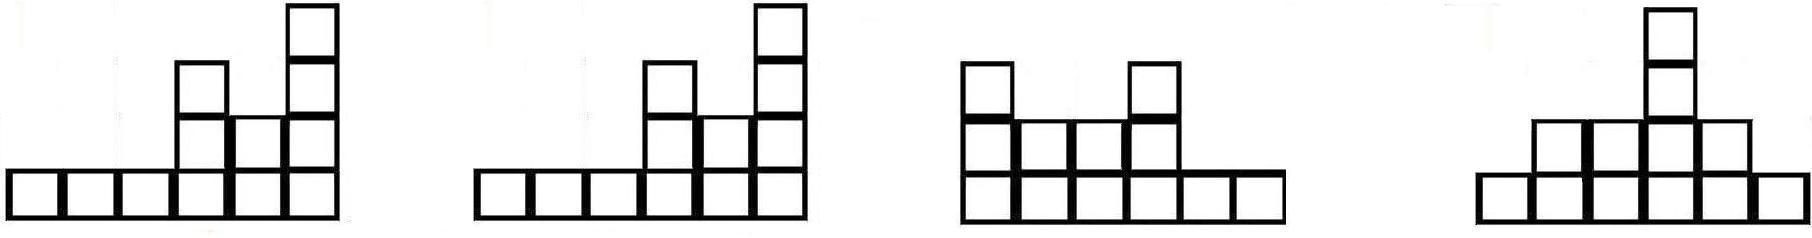
\includegraphics[height=2cm]{btz1.jpg}
\caption[Beispiel zum Brams,Taylor \& Zwicker Moving-Knife-Protokoll 1/5]{Boxendarstellungen des Kuchens f"ur die Spieler $p_1$, $p_2$, $p_3$ und $p_4$ (von links nach rechts)}
\end{figure}
\begin{figure}[h!]
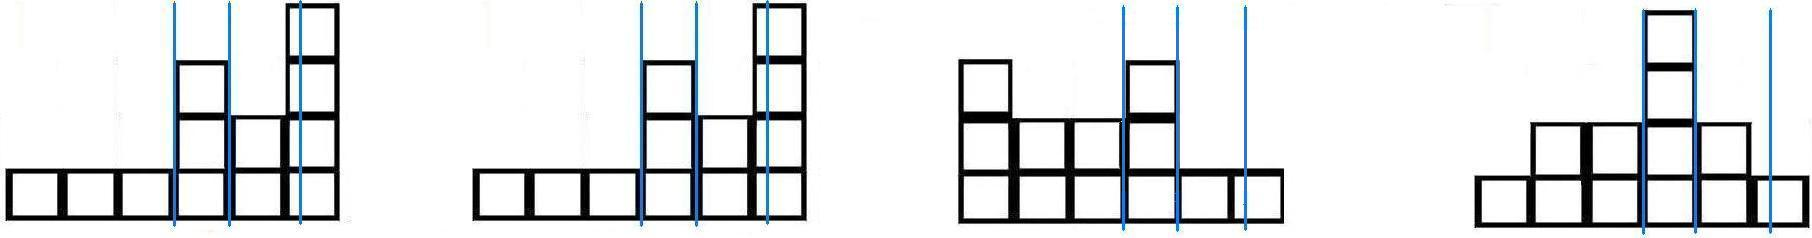
\includegraphics[height=2cm]{btz3.jpg}
\caption[Beispiel zum Brams,Taylor \& Zwicker Moving-Knife-Protokoll 2/5]{Die Spieler $p_1$ und $p_2$ teilen zusammen den Kuchen in vier gleichwertige St"ucke auf.}
\end{figure}
\begin{figure}[h!]
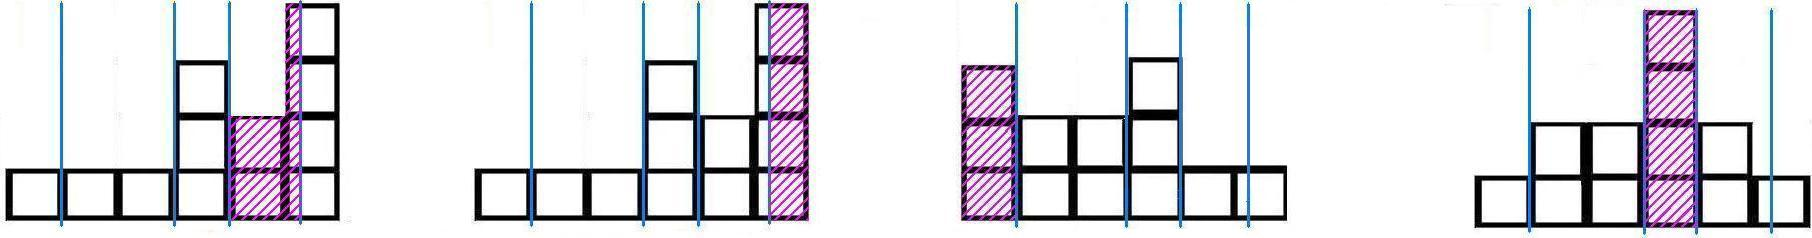
\includegraphics[height=2cm]{btz6.jpg}
\caption[Beispiel zum Brams,Taylor \& Zwicker Moving-Knife-Protokoll 3/5]{Der Spieler $p_3$ schneidet den Rest von dem wertvollsten St"uck ab (n.s.M.) und die Spieler $p_4,p_3,p_2,p_1$ w"ahlen (in dieser Reihenfolge) je ein St"uck aus.}
\end{figure}
\begin{figure}[h!]
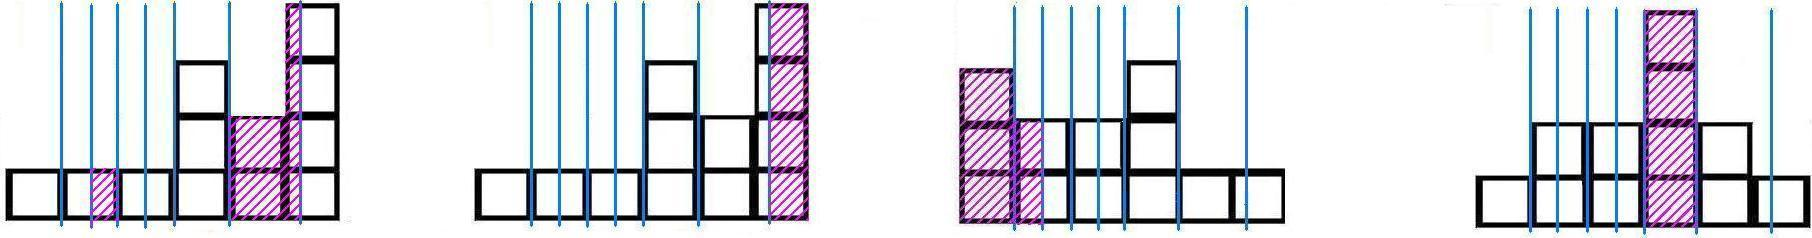
\includegraphics[height=2cm]{btz9.jpg}
\caption[Beispiel zum Brams,Taylor \& Zwicker Moving-Knife-Protokoll 4/5]{Es teilen $p_2$ und $p_4$ zusammen den Rest in vier gleichwertige St"ucke auf und die Spieler $p_3$ und $p_1$ w"ahlen (in dieser Reihenfolge) je ein Restst"uck aus.}
\end{figure}
\begin{figure}[h!]
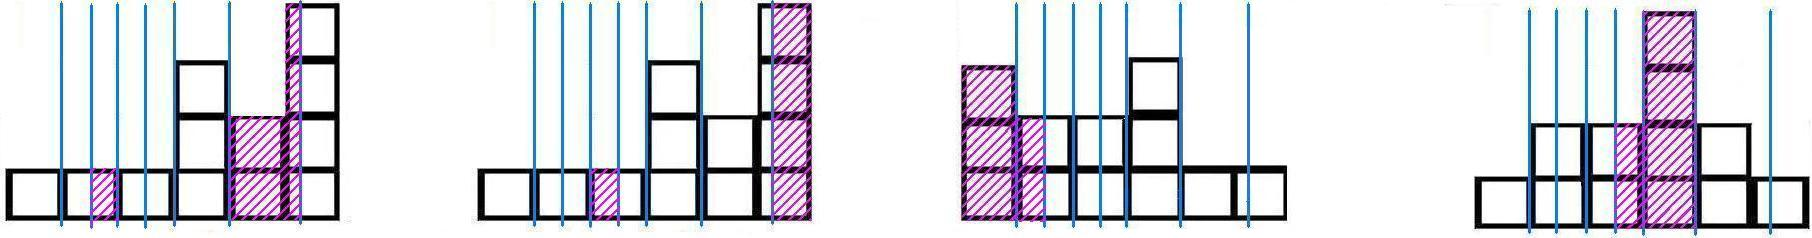
\includegraphics[height=2cm]{btz8.jpg}
\caption[Beispiel zum Brams,Taylor \& Zwicker Moving-Knife-Protokoll 5/5]{Die Spieler $p_2$ und $p_4$ nehmen je ein Restst"uck.}
\end{figure}
\end{bsp}
\newpage
\subsection{$n$ Spieler}
Es existiert ein endlich unbegrenztes, neidfreies Protokoll in \cite{5} f"ur eine beliebige Anzahl von Spielern.\\
Es folgt ein unendliches neidfreies Protokoll f"ur eine beliebige Anzahl von Spielern. Es wird hier f"ur $n=4$ aufgef"uhrt.\\
\newline
\begin{tabular}{|ll|}
\hline
&\textbf{Ein unendliches Protokoll}\\
\hline
\textbf{$\cdot$ Schritt 1}&Der erste Spieler $p_1$ schneidet den Kuchen $X$ in f"unf gleiche St"ucke (nach\\&seinem Ma"s). Der zweite Spieler $p_2$ sortiert diese als $X_1,X_2,X_3,X_4,X_5$\wf wtw\tf\\& mit:\\
&$v_1(X_1)=v_1(X_2)=v_1(X_3)=v_1(X_4)=v_1(X_5)=1/5$\\&$v_2(X_1) \geq v_2(X_2) \geq v_2(X_3)\geq v_2(X_4)\geq v_2(X_5)$\\
\textbf{$\cdot$ Schritt 2}&Ist $v_2(X_1)>v_2(X_3)$ oder $v_2(X_2)> v_2(X_3)$, so schneidet $p_2$ ggf. von $X_1$\\&und $X_2$ etwas ab, so dass er $X_1'=X_1-R_1$ und $X_2'=X_2-R_2$ erh"alt mit   \\&$v_2(X_1')=v_2(X_2')=v_2(X_3)$. Ist $v_2(X_1)=v_2(X_3)$ oder $v_2(X_2)=v_2(X_3)$, so\\&sei $X_1'=X_1$ und $X_2'=X_2$.\\
\textbf{$\cdot$ Schritt 3}&Der dritte Spieler $p_3$ sortiert $\{X_1',X_2',X_3,X_4,X_5\}$ als $Y_1,Y_2,Y_3,Y_4,Y_5$ mit:\\
&$v_3(Y_1) \geq v_3(Y_2) \geq v_3(Y_3)\geq v_3(Y_4)\geq v_3(Y_5)$\\
\textbf{$\cdot$ Schritt 4}&Ist $v_3(Y_1)>v_3(Y_2)$, so schneidet $p_3$ von $Y_1$ etwas ab, so dass er $Y_1'=$\\&$Y_1-R_3$ erh"alt mit $v_3(X_Y')=v_3(Y_2)$. Ist $v_3(Y_1)=v_3(Y_2)$, so sei  $Y_1'=Y_1$.\\
\textbf{$\cdot$ Schritt 5}&Aus $\{Y_1',Y_2,Y_3,Y_4,Y_5\}$ w"ahlen $p_4,p_3,p_2,p_1$ in dieser Reihenfolge je ein\\&St"uck. Falls solche St"ucke noch zur Wahl stehen, muss jeder Spieler eines\\&von den St"ucken nehmen, die er selber geschnitten hat.\\
\textbf{$\cdot$ Schritt 6}&Die Reste und das "ubriggebliebene St"uck werden verschmolzen und das\\&Protokoll kann beliebig oft wiederholt werden.\\
\hline
\end{tabular}
\newline
\newline
\newline
Das folgende Protokoll l"asst sich verallgemeinern, indem die Anzahl der St"ucke in welche der erste Spieler in Schritt 1 den Kuchen teilt immer um zwei gr"osser ist als die Summe der Schnitte ab Schritt 2 und bis zu dem Analogon von Schritt 5 ("ublicherweise von Schritt 2 bis Schritt (2$\cdot n$-3) ). Es muss davon ausgegangen werden, dass alle Spieler die M"oglichkeit haben m"ussen unterschiedliche St"ucke beschneiden zu k"onnen. Somit wird einkalkuliert, dass der letzte Spieler $p_n$ ein unbeschnittenes St"uck nehmen kann und f"ur den Spieler $p_1$ ein unbeschnittenes St"uck "ubrig bleiben muss. Der $i$-te Spieler mit $2 \leq i \leq (n-1)$ darf immer $n-i$ St"ucke beschneiden.\\
Bemerkung: Es bleibt nach jedem Schritt ein Rest "ubrig.
\begin{bsp}\wf rfsdf
\begin{figure}[h!]
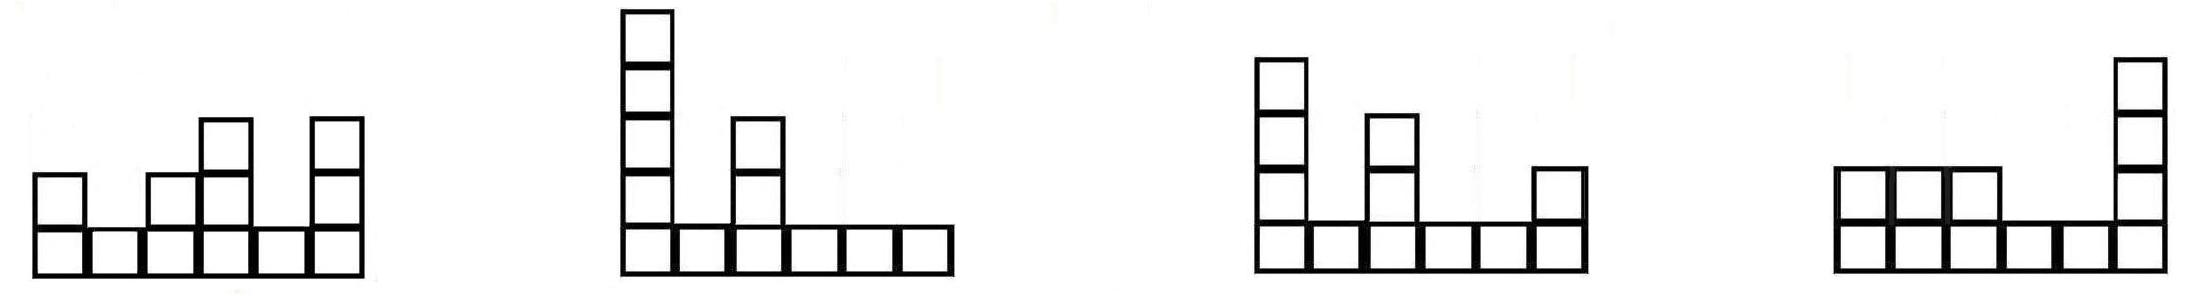
\includegraphics[height=2cm]{upfv.jpg}
\caption[Beispiel zum unendlichen Protokoll 1/4]{Boxendarstellungen des Kuchens f"ur die Spieler $p_1$, $p_2$, $p_3$ und $p_4$ (v.l.n.r.)}
\end{figure}
\begin{figure}[h!]
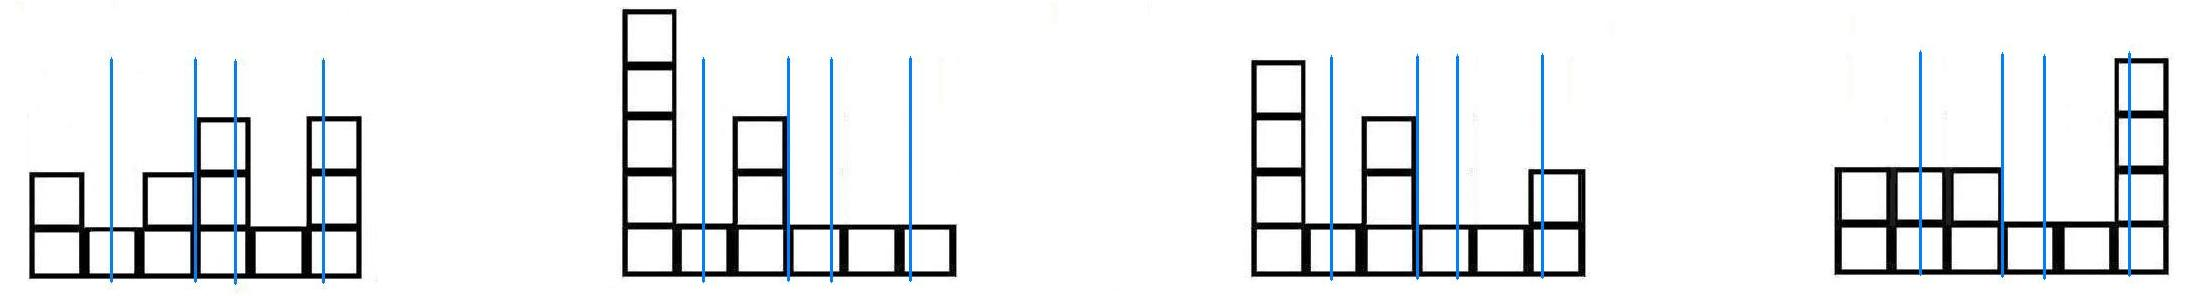
\includegraphics[height=2cm]{upfv2.jpg}
\caption[Beispiel zum unendlichen Protokoll 2/4]{Der Spieler $p_1$ viertelt den Kuchen (n.s.M.).}
\end{figure}
\begin{figure}[h!]
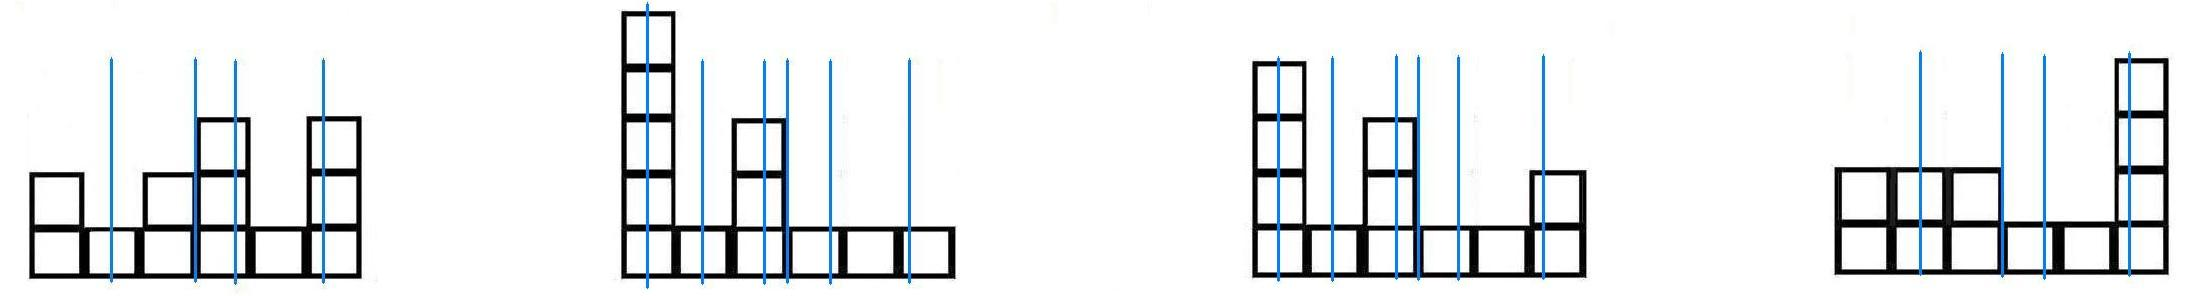
\includegraphics[height=2cm]{upfv3.jpg}
\caption[Beispiel zum unendlichen Protokoll 3/4]{Der Spieler $p_2$ schneidet je einen Rest von seinen zwei wertvollsten St"ucken. Der Spieler $p_3$ muss damit kein St"uck mehr beschneiden.}
\end{figure}
\begin{figure}[h!]
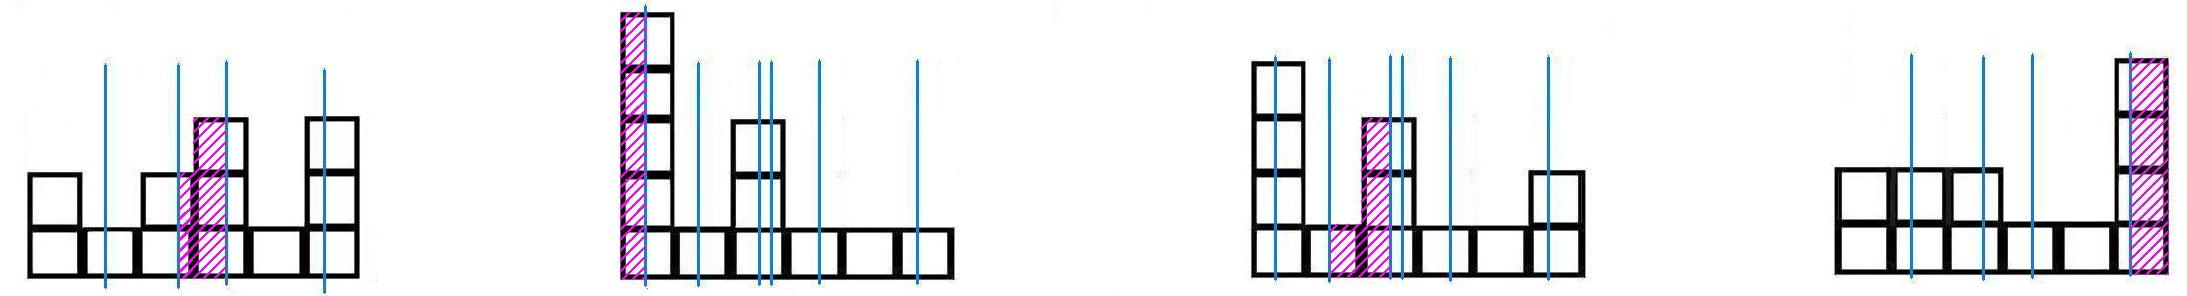
\includegraphics[height=2cm]{upfv5.jpg}
\caption[Beispiel zum unendlichen Protokoll 4/4]{Die Spieler $p_4,p_3,p_2,p_1$ w"ahlen (in dieser Reihenfolge) je ein St"uck aus.}
\end{figure}
\end{bsp}\newpage
Wie bereits gesehen, gibt es auch Protokolle die keine komplette Aufteilung liefern, aber in der Teilaufteilung neidfrei sind. So k"onnte man solche Teilaufteilungen untersuchen und versuchen zu vereinen. Durch die Additivit"at von Bewertungen bleiben solche Verfahren neidfrei. Dabei kann man auch von einem vorgegebenen Zustand ausgehen und den Kuchen bis zum Ende aufteilen. So gibt es eine neidfreie Aufteilung f"ur f"unf Spieler, wenn man aus einem neidfreien Zustand ausgeht, der eine bestimmte Eigenschaft erf"ullt. Das genaue Vorgehen wird in \cite{21} geschildert.\\
\newline
\newline
Es folgt ein kontinuierliches, exaktes Protokoll aus \cite{20} f"ur eine beliebige Anzahl von Spielern. Austin selbst hat es am Beispiel f"ur $n=3$ ausformuliert.\\
\newline
\begin{tabular}{|ll|}
\hline
&\textbf{Austin exaktes Protokoll}\\
\hline
\textbf{$\cdot$ Runde 1}&Der Spieler $p_1$ und Spieler $p_2$ benutzen AMKP und bekommen:\\&$v_1(X_1)=v_1(X_2)=1/2$ und $v_2(X_1)= v_2(X_2)=1/2.$\\
\textbf{$\cdot$ Runde 2}&Der Spieler $p_1$ und Spieler $p_3$ benutzen AMKP3\abk{AMKP$n$}{\markup{A}ustin \markup{M}oving-\markup{K}nife-\markup{P}rotokoll f"ur $\markup{n}$ gleichwertige St"ucke} und bekommen\\&ein St"uck mit der Eigenschaft:\\&$v_1(X_{11})=1/3 \cdot v_1(X_1)= v_3(X_{11})=1/3 \cdot v_3(X_1).$\\&Der Spieler $p_2$ und Spieler $p_3$ benutzen AMKP3 und bekommen:\\&$v_2(X_{21})=1/3 \cdot v_2(X_2)=v_3(X_{21})=1/3 \cdot v_3(X_2).$\\&
Dannach bekommt der Spieler $p_3$ jeweils die St"ucke von den\\&Aufteilungen und diese werden zu $X_3$ verschmolzen. Die "ubrigen\\&zwei St"ucke werden wieder als $X_1$ und $X_2$ bezeichnet.\\ 
\textbf{$\cdot$ Runde $\cdots$}&$\cdots$\\
\textbf{$\cdot$ Runde $n-1$}&Der Spieler $p_1$ und Spieler $p_n$ benutzen AMKPn und bekommen:\\&$v_1(X_{11})=1/n \cdot v_1(X_1)=v_n(X_{11})=1/n \cdot v_n(X_1).$\\&Der Spieler $p_2$ und Spieler $p_n$ benutzen AMKP3 und bekommen:\\&$v_2(X_{21})=1/n \cdot v_2(X_2)=v_n(X_{21})=1/n \cdot v_n(X_2).$\\& $\cdots$\\&Der Spieler $p_{n-1}$ und Spieler $p_n$ benutzen AMKPn und bekommen:\\&$v_{n-1}(X_{(n-1)1})=1/n \cdot v_{n-1}(X_{n-1})=v_n(X_{(n-1)1})=1/n \cdot v_n(X_{n-1}).$\\&
Der Spieler $p_n$ bekommt jeweils die St"ucke von den Aufteilungen.\wf fffffffff\tf\\
\hline
\end{tabular}
\newline
\newline
\newline
Das Protokoll ist exakt, denn der $n$-te Spieler bekommt $$1/n\cdot v_n(X_1)+1/n\cdot v_n(X_2)+\cdots+1/n\cdot v_n(X_{n-1})=1/n\cdot(v_n(X_1)+v_n(X_2)+\cdots+\cdot v_n(X_{n-1}))$$ $$=^{Additivit"at}1/n\cdot v_n(X_1+X_2+\cdots+X_{n-1})=1/n \cdot 1=1/n$$ und jeder $i$-te Spieler mit $1 \leq i \leq (n-1)$ beh"alt den $(n-1)/n$ Anteil von seinem St"uck mit dem jeweiligen Wert $1/(n-1)$. Also $$(n-1)\cdot 1/{n\cdot 1/(n-1)}=1/n$$.\\
Dieses Protokoll ist nicht neidfrei, da aus der Exaktheit keine Neidfreiheit folgt. Durch eine einfache Modifikation kann dieses Protokoll f"ur $n \leq 4$ neidfrei gemacht werden.
Das Vorgehen bleibt gleich, bis auf die Tatsache, dass sich der Spieler aus jeder Ausf"uhrung von AMKP, wo er nicht beteiligt war, das wertvollste St"uck nehmen muss. Bei Runde 1 w"are dies Cut \& Choose. Bei Runde 2 muss Spieler $p_2$ ein St"uck von Spieler $p_1$ und Spieler $p_1$ ein St"uck  von Spieler $p_2$ nehmen. Bei Runde 3 k"onnten drei Reste entstehen, welche aber nach dem Prinzip vom Brams, Taylor \& Zwicker-Protokoll neidfrei aufgeteilt werden k"onnten.\\Bei Runde 4 und f"unf Spieler entsteht wieder das bekannte Problem. Hier k"onnte aber eine L"osung m"oglich sein, in dem man die Aufteilung in zwei Schritte spaltet, und im ersten die St"ucke unter den Spielern die bereits ein St"uck haben aufteilt, und in der zweiten den neu dazukommenden Spieler $p_5$ beachtet. Das AMKP f"uhren nun die Spieler mit St"ucken untereinander aus. Dieses Protokoll k"onnte eine kontinuierliche Verallgemeinerung auf $n$ Spieler der neidfreien Protokolle liefern.\\ 
\section{Komplexit"at von Protokollen}
\subsection{Anfragemodell nach J. Robertson und W. Webb}
\textbf{Erinerung:}\\
Ein Protokoll hat am Anfang keine Informationen "uber die Bewertungen der Spieler, bis auf die Normalisierung. Der Kuchen $X$ wird durch das Intervall $[0,1]\subseteq \mathbb{R}$ repr"asentiert. F"ur ein $\alpha \in \mathbb{R}$ mit $0 \leq \alpha \leq 1$ bezeichnet man als einen \underline{$\alpha$-Punkt} vom Spieler $p_i$ f"ur $p_i \in P_N$ die kleinste Zahl $x$ mit der Eigenschaft $v_i([0,x])=\alpha$ (aus den Eigenschaften der Bewertung folgt $v_i([x,1])=1-\alpha$).
\begin{defi}[Anfragen im Robertson-Webb Modell]\footnote{vgl. \cite{50}} \wf rgkhbr \tf \\
\begin{itemize}
\item Schnitt($p_i;\alpha$): Der Spieler $p_i$ macht einen Schnitt in seinem $\alpha$-Punkt. Der Wert $x$ wird an das Protokoll zur"uckgegeben.\\
\item Bewertung($p_i;x$): Der Spieler $p_i$ bewertet den Schnitt $x$ ($x$ ist dabei ein Schnitt, welcher zuvor vom Protokoll ausgef"uhrt wurde). Dieser Wert $v_i(x)$ wird an das Protokoll zur"uckgegeben.\\
\item Zuordnung($p_i;x_i,x_j$): Dem Spieler $p_i$ wird das Intervall $[x_i,x_j]$ ($x_i \leq x_j$ sind zwei zuvor ausgef"uhrte Schnitte vom Protokoll oder 0 oder 1) zugeordnet. Alle solche Intervalle sind disjunkt.
\end{itemize}  
\end{defi}
Die \underline{Komplexit"at eines Protokolls} ist die Summe der Anzahlen der Schnitte und Bewertungen im ung"unstigsten Fall.\newpage
\subsection{Resultat von M. Magdon-Ismail, C. Busch und\\M. S. Krishnamoorthy}
Es wurden zwei Theoreme "uber die unteren Schranken von starken und super-neidfreien Cake-Cutting-Protokolle in \cite{6} bewiesen.
\begin{thm}(Untere Schranke von starken neidfreien Protokollen)
\newline Es gibt Bewertungsfunktionen, f"ur welche ein starkes neidfreies Cake-Cutting-Protokoll die Komplexit"at $\Omega(0.086\cdot n^2)$ besitzt.
\end{thm}
\begin{thm}(Untere Schranke von super-neidfreien Protokollen)
\newline Es gibt Bewertungsfunktionen f"ur welche ein super-neidfreies Cake-Cutting-Protokoll die Komplexit"at $\Omega(0.25\cdot n^2)$ besitzt.
\end{thm}
Das Resultat zeigt bereits einen Unterschied zu den proportionalen Protokollen ($\mathcal{O}(n$log$ n)$ aus \cite{3}), ist aber leider sehr schwach, da starke und super-neidfreie Cake-Cutting-Protokolle sehr starke Einschr"ankungen sind, und nicht immer existieren. Dagegen lieferte das folgende Theorem die lang vermutete endg"ultige Separation von der Proportionalit"at.
\subsection{Resultat von A. Procaccia}
In der Arbeit \cite{9} wird ein neues kompliziertes Problem formuliert und gezeigt, dass eine Aufteilung nur dann neidfrei ist, wenn das Problem eine L"osung hat. Eine L"osung daf"ur zu finden liegt in $\Omega( n^2)$ und daraus folgt:
\begin{thm} \wf jbdfksdbfksd\\ \tf
Die Anfragekomplexit"at (im Robertson-Webb-Modell) f"ur eine neidfreie Aufteilung betr"agt $\Omega(n^2)$.
\end{thm}
\textbf{Die Idee:}\\
Die Aufgabe von jedem Spieler ist es einzeln und unabh"angig von den anderen Spielern den Kuchen in Intervalle $I$ zu unterteilen. F"ur jedes $I=[x_1,x_2]$ mit $x_1,x_2 \in [0,1]$ ist die L"ange $|I|=x_2-x_1$. Solche Intervalle werden in $\Pi_k^i$ mit $i \in \mathbb{N}$ f"ur jeweils den $p_i$-ten Spieler und $k \in \mathbb{N}$, f"ur die $k$-te Etappe der Gliederung, dargestellt. Das Einteilen in Intervalle ist gleich dem Anfragemodell von Robertson und Webb. Es gibt auch gleichzeitige Bewertungen von zwei Schnitten: Bewertung($p_i;x_1,x_2$). Dabei werden die Werte $v_i(0,x_1),v_i(x_1,x_2)$ und $v_i(x_2,1)$ an das Protokoll zur"uckgegeben.
\\Wenn zwei Eigenschaften erf"ullt werden, erfolgt eine Aufteilung der St"ucke unter den Spieler.\\Die erste Eigenschaft muss f"ur die H"alfte der Spieler gelten, welche gew"ahrleisten m"ussen, dass ihre Portion, welche aus einem oder mehreren Intervallen besteht, h"ochstens die L"ange $2/n$ hat. Ansonsten h"atte der gesamte Kuchen eine L"ange gr"osser $1$.\\Die zweite Eigenschaft nennt sich ausschlaggebend (critical). Nur wenn die Portionen ausschlaggebend sind, kann eine Aufteilung neidfrei sein. Ein ausschlagebendes St"uck muss aus Intervallen bestehen deren Wertesumme mindestens so gross ist, wie der Wert von jedem anderen Intervall w"ahrend der Aufteilung. Denn g"abe es ein Intervall, das mehr Wert ist als das betrachtete St"uck (potentielle Portion), so w"urde es ein Gegenspieler bekommen, und es w"urde Neid entstehen.\\F"ur die Komplexit"at gilt: Mindestens $n/4$ Ausf"uhrungen der Aufteilung werden gebraucht um Intervalle mit h"ochstens der L"ange $2/n$ zu bekommen. Diese Anzahl folgt aus der Durchf"uhrung (siehe Beispiel), denn es lassen sich h"ochstens zwei zus"atzliche Intervalle in einer Etappe der Gliederung erzeugen. Damit kann nach $n/4-1$ Ausf"uhrungen der Kuchen aus h"ochstens $Anzahl$ $neuer$ $Intervalle$ $pro$ $Ausf"uhrung \cdot Anzahl$ $Ausf"uhrungen + Anzahl$ $Intervalle$ $im$ $Anfangszustand= 2 \cdot (n/4-1)+1= n/2-1$ St"ucken bestehen. Also muss mind. ein Intervall eine L"ange von mehr als $2/n$ haben, sonst w"are die L"ange des gesamten Kuchens kleiner als $1$. Sei die Bewertung von allen Spielern von einem St"uck immer gleich seiner L"ange. Es gilt, dass bevor nicht alle Intervalle eine L"ange kleiner $2/n$ haben, gibt es Spieler mit einer nicht ausschlaggebenden Portion und damit kann die Aufteilung nicht neidfrei sein. Es reicht einen solchen Fall zu betrachten, denn eine untere Schranke muss f"ur alle m"oglichen Bewertungen gelten. Damit gilt f"ur die Komplexit"at $\Omega(Anzahl Spieler \cdot Anzahl Ausf"uhrungen)=\Omega(n/2 \cdot n/4)=\Omega(n^2)$.\\ \newline
\textbf{Veranschaulichung an einem Beispiel:}\\
Man f"uhrt solange Schnitt- und Bewertungsanfragen aus bis mindestens f"ur $n/2$ Spieler Intervalle der L"ange kleiner gleich $2/n$ gibt und diese werden untersucht, ob sie ausschlaggebend sind. Die L"ange der Intervalle muss bei jedem Spieler kleiner gleich der L"ange seiner Portion sein, da jedes St"uck Kuchen die Vereinigung von endlich vielen disjunkten Intervallen ist. Bevor man versucht den Kuchen aufzuteilen, muss jeder Spieler mindestens eine Anfrage ausgef"uhrt haben.\\
\newline
Beispiel f"ur vier Spieler mit mindestens drei Schnitten:
\begin{itemize}
\item Ausgangssituation: $\Pi_1^0=\{[0,1]\}$, $\Pi_2^0=\{[0,1]\}$, $\Pi_3^0=\{[0,1]\}$, $\Pi_4^0=\{[0,1]\}$
\item  Schnitt($p_1;1/3$)=$1/4$ Der erste Spieler hat ein St"uck, dessen L"ange kleiner gleich 1/2 ist. Dieses St"uck ist nicht ausschlaggebend.\\$\Pi_1^1=\{[0,1/4],[1/4,1]\}$, $\Pi_2^1=\{[0,1]\}$, $\Pi_3^1=\{[0,1]\}$, $\Pi_4^1=\{[0,1]\}$
\item  Schnitt($p_2;1/2$)=$3/4$ Der zweite Spieler hat ein St"uck, dessen L"ange kleiner gleich 1/2 ist. Dieses St"uck ist ausschlaggebend.\\$\Pi_1^2=\{[0,1/4],[1/4,1]\}$, $\Pi_2^2=\{[0,3/4],[3/4,1]\}$, $\Pi_3^2=\{[0,1]\}$, $\Pi_4^2=\{[0,1]\}$
\item  Bewertung($p_3;[1/4,3/4]$)=$7/8$, Protokoll erf"ahrt zus"atzlich $v_3([0,1/4])=1/16$ und $v_3([3/4,1])=1/16$.\\ $\Pi_1^3=\{[0,1/4],[1/4,1]\}$, $\Pi_2^3=\{[0,3/4],[3/4,1]\}$, $\Pi_3^3=\{[0,1/4],[1/4,3/4],[3/4,1]\}$, $\Pi_4^3=\{[0,1]\}$
\item  Schnitt($p_4;1/2$)=$1/2$ (Das Minimum der Schnitte wurde erreicht und alle Spieler haben den Kuchen geschnitten oder bewertet.)\\ $\Pi_1^4=\{[0,1/4],[1/4,1]\}$, $\Pi_2^4=\{[0,3/4],[3/4,1]\}$, $\Pi_3^4=\{[0,1/4],[1/4,3/4],[3/4,1]\}$, $\Pi_4^4=\{[0,1/2],[1/2,1]\}$
\item Spieler $p_3$ und $p_4$ haben aber keine ausschlaggebenden St"ucke, denn es wurde noch kein passendes St"uck f"ur diese Spieler gefunden.
\item  Bewertung($p_4;[1/4,3/4]$)=$7/10$, Protokoll erf"ahrt zus"atzlich $v_4([0,1/4])=1/10$, $v_4([1/4,1/2])=4/10$, $v_4([1/2,3/4])=3/10$ und $v_4([3/4,1])=2/10$.\\ $\Pi_1^5=\{[0,1/4],[1/4,1]\}$, $\Pi_2^5=\{[0,3/4],[3/4,1]\}$, $\Pi_3^5=\{[0,1/4],[1/4,3/4],[3/4,1]\}$, $\Pi_4^5=\{[0,1/4],[1/4,1/2],[1/2,3/4],[3/4,1]\}$
\begin{figure}[h!]
\center
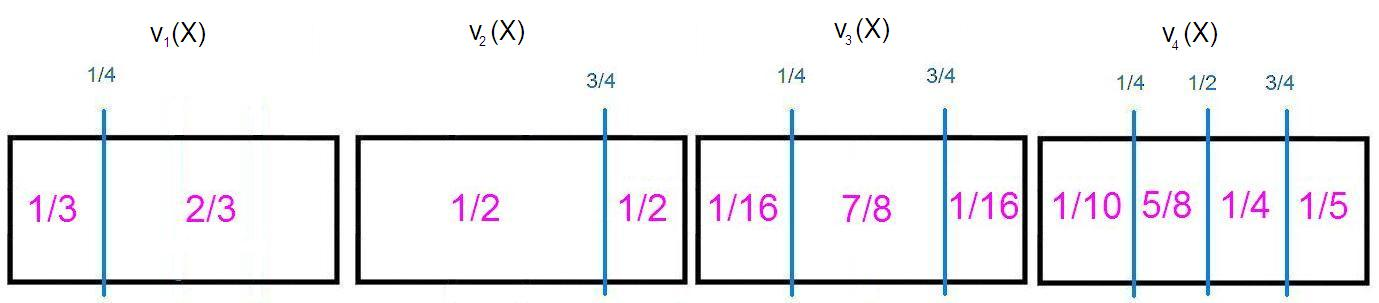
\includegraphics[height=3cm]{kk5.jpg}
\caption[Beispiel zu Procaccias Teilungsspiel 1/2]{Der Kenntnisstand des Protokolls in dieser Etappe.}
\end{figure}  
\item Bewertung($p_3;[1/4,1/2]$)=$5/8$, Protokoll erf"ahrt zus"atzlich $v_3([1/2,3/4])=2/8$. Nun ist das St"uck von Spieler $p_3$  auch ausschlaggebend.\\ $\Pi_1^6=\{[0,1/4],[1/4,1]\}$, $\Pi_2^6=\{[0,3/4],[3/4,1]\}$, $\Pi_3^6=\{[0,1/4],[1/4,1/2],[1/2,3/4],$\\ $[3/4,1]\}$, $\Pi_4^6=\{[0,1/4],[1/4,1/2],[1/2,3/4],[3/4,1]\}$
\item Der Spieler $p_1$ w"urde das St"uck $X_1$ bekommen. Dieses St"uck ist nicht ausschlaggebend, denn f"ur das Intervall $I_1$ gilt $1/3=v_1(X_1)<v_1(X-X_1)=2/3$, damit k"onnten $X_4, X_3$ oder $X_2$ mehr Wert sein (n.s.M.). Also wird ein weiterer Schritt ausgef"uhrt.
\item  Bewertung($p_1;[1/2,3/4]$)=$1/4$, Protokoll erf"ahrt zus"atzlich $v_1([1/4,1/2])=1/6$ und $v_1([3/4,1])=1/4$ \\ $\Pi_1^7=\{[0,1/4],[1/4,1/2],[1/2,3/4],[3/4,1]\}$, $\Pi_2^7=\{[0,3/4],[3/4,1]\}$, $\Pi_3^7=\{[0,1/4],[1/4,1/2],[1/2,3/4],[3/4,1]\}$, $\Pi_4^7=\{[0,1/4],[1/4,1/2],[1/2,3/4],[3/4,1]\}$
\item Nun sind alle St"ucke ausschlaggebend und "uber die H"alfte der Spieler haben Intervalle mit der L"ange kleiner gleich $1/2$. Also liegt einer Aufteilung nichts mehr im Wege und diese wird ausgef"uhrt. Die Bewertungen der einzelnen St"ucke werden aufgelistet:\\
\newline
\begin{tabular}{llll}
$v_1(X_1)=1/3$ & $v_1(X_4)=1/6$ & $v_1(X_3)=1/4$ & $v_1(X_2)=1/4$\\
$v_2(X_1)\leq1/2$ & $v_2(X_4)\leq1/2$ & $v_2(X_3)\leq1/2$ & $v_2(X_2)=1/2$\\
$v_3(X_1)=1/16$ & $v_3(X_4)=5/8$ & $v_3(X_3)=1/4$ & $v_3(X_2)=1/16$\\
$v_4(X_1)=1/10$ & $v_4(X_4)=2/5$ & $v_4(X_3)=3/10$ & $v_4(X_2)=1/5$
\end{tabular}
\begin{figure}[h!]
\center
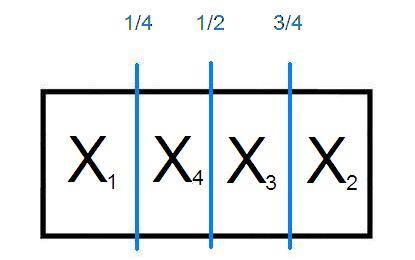
\includegraphics[height=4cm]{kk4.jpg}
\caption[Beispiel zu Procaccias Teilungsspiel]{Die Endaufteilung}
\end{figure}  
\end{itemize}\newpage
\section{Zusammenfassung und Ausblick}
In dieser Arbeit wurde eine Einf"uhrung in die Problematik des neidfreien Teilens gegeben. Es wurden alle wichtigen endlich beschr"ankten neidfreien Protokolle mit parallelen Schnitten auf einem rechteckigen Kuchen ausf"uhrlich behandelt und anhand von Beispielen erl"autert. Dabei wurden zwei M"oglichkeiten gefunden inwiefern sich in Zukunft eine Verallgemeinerung auf eine beliebige Anzahl von Spielern erm"oglichen k"onnte. Ausserdem wurde die f"ur die Komplexit"atsanalyse von neidfreien Cake-Cutting-Protokollen wichtige Aussage von Ariel Procaccia erkl"art und an einem Beispiel demonstriert.\\Eine weitere in diesem Kontext interessante Frage, die sich stellt ist die Aufteilung mit Vollmachten. So "ubertragen z.B. ein Teil der Spieler ihre Vollmacht an einen Verantwortlichen, dieser sieht ihre Bewertungen und kann somit Ihnen St"ucke zuordnen. Hier untersuche man, ob die Neidfreiheit leichter oder schwieriger erreicht werden kann. Au"serdem kann nun in Abh"angigkeit der Ehrlichkeit des Verantwortlichen die Effizienz der Aufteilungen gepr"uft werden. Es kann auch gepr"uft werden, wie sich die Aufteilung entwickelt, wenn ein Spieler die Vollmacht von allen anderen hat. Oder wenn mehrere Spieler Vollmachtbeauftragte sind z.B. bei einer Scheidung, wo eines der Kind die Vollmacht auf beide Elternteile "ubertr"agt.\\
\newpage
\thispagestyle{empty}
\thispagestyle{plain}
\renewcommand{\refname}{Literaturverzeichnis}
\addcontentsline{toc}{section}{Literaturverzeichnis}
\begin{thebibliography}{9}
\bibitem[Aus82]{20} A. K. Austin. Sharing a Cake. \emph{Mathematikal Gazette}, 66, 1982.
\bibitem[BB04]{40} J. B. Barbanel and S. J. Brams, Cake Division with Minimal Cuts: Envy-Free Procedures for 3 Persons, 4 Persons, and Beyond.\emph{Math. Social Sciences 48}: 251-269, 2004.
\bibitem[BT96]{26} S. Brams and A. Taylor. \emph{Fair Division: From Cake-Cutting to Dispute Resolution}. Cambridge University Press, 1996.
\bibitem[BTZ97]{5} S. J. Brams, A. D. Taylor, and W. S.
Zwicker. A moving-knife solution to the four-person envy
free cake division problem. \emph{Proceedings of the American
Mathematical Society}, 125(2):547-554, 1997.
\bibitem[CLPD10]{23} Y. Chen, J. Lai, D. Parkes, and A. Procaccia. Truth, Justice, and Cake Cutting. \emph{In the Proceedings 24th AAAI Conference on Artificial Intelligence (AAAI '10)}, 2010.
\bibitem[CNS10]{1} J. Cloutier, C. Nyman and F. Su. Two-Player Envy-Free Multi-Cake Division.\emph{Mathematical Social Sciences}
Volume 59, Issue 1, Pages 26-37, 2010. 
\bibitem[End09]{36} Ulle Endriss. Lecture Notes on Fair Division. ILLC, University of Amsterdam, September 2009.
\bibitem[EP84]{3} S. Even and A. Paz. A note on cake-cutting. \emph{Discrete Applied Mathematics}, 7:285-296, 1984.
\bibitem[EP06]{30} J. Edmonds and K. Pruhs. Cake
cutting really is not a piece of cake. In\emph{Proceedings of
the 17th Annual ACM-SIAM Symposium on Discrete Algorithms (SODA)}, pages 271-278, 2006.
\bibitem [Fol67]{8} D. Foley, Resource allocation and the public sector,\emph{Yale Economic Essays 7},45-98,1967.
\bibitem [GS58]{18} G. Gamow and M. Stern.\emph{Puzzle-Math.}Viking, New York, 1958.
\bibitem[HS05]{25} C.- J. Haake and F. Su. Fair Division Procedures: Why use Mathematics?\emph{Procedural Approaches to Conflict Resolution}, M. Raith (ed.), Springer Verlag, 2005.
\bibitem[Jon07]{31} M. A. Jones. Some Recent Results on Pie Cutting. Fair Division,\emph{Dagstuhl Seminar Proceedings} 2007.
\bibitem [Kna46]{7} B.  Knaster,  Sur  le  probleme  du  partage  pragmatique  de  H.  Steinhaus,\emph{Ann.  Soc.  Polon.  Math.}19 (1946), 228-230. 
\bibitem[LR09]{53} C. Lindner and J. Rothe. Degrees of Guaranteed Envy-Freeness in Finite Bounded Cake-Cutting Protocols. \emph{Proceedings of the 5th Workshop on Internet \& Network Economics (WINE 2009)}, Rome, Italy. Springer-Verlag Lecture Notes in Computer Science 5929, pages 149-159, 2009.
\bibitem[MIBK03]{34} M. Magdon-Ismail, C. Busch, and M. Krishnamoorthy. Cake-cutting is not a piece of cake. In \emph{Proceedings of the 20th Annual Symposium on Theoretical Aspects of Computer Science}, pages 596-607. Springer-Verlag Lecture Notes in Computer Science \#2607, 2003.
\bibitem[MIBK05]{6} M.Magdon-Ismail, C. Busch, and
M. S. Krishnamoorthy. Hardness results for cake cutting. \emph{Bulletin of the EATCS}, 86:85-106, 2005
\bibitem[Pro09]{9} A. Procaccia. Thou shalt covet thy neighbor's cake. In \emph{Proceedings of the 21st International Joint Conference on Artificial Intelligence}, pages 239-244. IJCAI, July 2009.
\bibitem[Rot08]{19} J. Rothe,\emph{Komplexit"atstheorie und Kryptologie: Eine Einf"uhrung in Kryptokomplexit"at} Springer, Berlin. 2008.
\bibitem[Rot10]{28} J. Rothe, Cake-Cutting Algorithms, D"usseldorf, WS 2009/2010.
\bibitem[RW95]{35} J. M. Robertson and W. A. Webb. Approximating fair division with a limited number of cuts, \emph{Journal of Combinatorial Theory}, Series A 72, 340-344, 1995.
\bibitem[RW98]{27} J. Robertson and W. Webb. \emph{Cake-Cutting Algorithms: Be Fair If You Can}. A K Peters, 1998.
\bibitem[Ste48]{17} H. Steinhaus. The problem of fair division. \emph{Econometrica}, 16:101-104, 1948.
\bibitem[Su99]{11} F. Su. Rental harmony: Sperner's lemma in fair division. \emph{Amer. Math. Monthly}, 106(10):930-942, 1999.
\bibitem[SW09]{21} A. Saberi and Y. Wang. Cutting a Cake for Five People. \emph{AAIM '09: Proceedings of the 5th International Conference on Algorithmic Aspects in Information and Management}, pages 292-300. Springer-Verlag.2009.
\bibitem[Var74]{52} H. Varian. Equity, envy, and efficiency. \emph{Journal of Economic Theory}, 9(1):63-91, 1974.
\bibitem[Wal10]{41} T. Walsh. Online Cake Cutting. \emph{COMSOC'10: Third International Workshop on Computational Social Choice}, pages 247-258. D"usseldorf University Press.2010.
\bibitem[WS03]{50} G. J. Woeginger and J. Sgall. A Lower Bound for Cake Cutting,\emph{In European Symposium on Algorithms (ESA}, pages 459-469, 2003.
\bibitem[WS07]{24} G. J. Woeginger and J. Sgall.
On the complexity of cake cutting. \emph{Discrete Optimization},
4:213-220, 2007.
\bibitem[Zen00]{12} D. Zeng. Approximate Envy-Free Procedures. \emph{Game Practice: Contributions from Applied Game Theory.} Kluwer Academic Publishers, Dordrecht, pp. 259-271, 2000.
\end{thebibliography}
\newpage
\thispagestyle{empty}
\tf
\begin{center}
\Huge Erkl"arung
\end{center}
\vspace{1cm}
\noindent Hiermit versichere ich, die vorliegende Bachelorarbeit selbstst"andig verfasst und keine anderen als die angegebenen Quellen und Hilfsmittel benutzt zu haben.\\
\vspace{3cm}\\
D"usseldorf, 21. September 2010 \hfill Alina Elterman

\end{document}
